\begin{chapter}{Vectores}\label{chap-vectores}

    El concepto de vector es básico para el estudio de funciones de varias variables y proporciona la motivación geométrica para todo el curso. Por lo tanto, las propiedades de los vectores, tanto algebraicas como geométricas, serán discutidas en forma resumida en este capítulo.
    
    \begin{section}{\'Algebra lineal en $\R^2$ y $\R^3$}\label{seccion-algebra-lineal-en-R2-yR3}  
        Sabemos que se puede usar un número para representar un punto en una línea, una vez que se selecciona la longitud de una unidad.
        
        \begin{figure}[h]\label{fig-punto-en-R}
            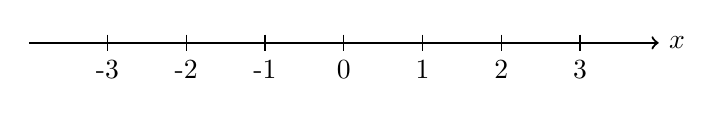
\begin{tikzpicture}
            \draw[thick,->] (-4.0,0) -- (4.0,0) node[right] {$x$}; % eje x
            \foreach \x in {-3,...,3}
            \draw (\x,3pt) -- (\x,-3pt)
            node[anchor=north] {\x};
            \end{tikzpicture}
            \caption{La recta real y algunos números enteros.}
        \end{figure}

        Se puede usar un par de números $(x, y)$ para representar un punto en el plano. Estos pueden ser representados como en la figura \ref{fig-punto-en-R2}.
        \begin{figure}[h]
        	\centering
            \begin{tikzpicture}
            \draw[thick,->] (-4.0,0) -- (4.0,0) node[right] {$x$}; % eje x
            \draw[thick,->] (0,-3) -- (0,3) node[above] {$y$}; % eje y
            \foreach \x in {-3,...,-1}
            \draw (\x,3pt) -- (\x,-3pt)
            node[anchor=north] {\x};
            \foreach \x in {1,...,3}
            \draw (\x,3pt) -- (\x,-3pt)
            node[anchor=north] {\x};
            \foreach \y in {-2,...,-1}
            \draw (3pt,\y) -- (-3pt,\y) 
            node[anchor=east] {\y}; 
            \foreach \y in {1,...,2}
            \draw (3pt,\y) -- (-3pt,\y)
            node[anchor=east] {\y}; 
            \draw[fill] (2,1) circle [radius=0.07];
            %\draw[thick,->] (0,0) -- (2,1);
            \node [right] at (2,1) {$(2,1)$};
            \draw [dashed] (0,1) -- (2,1);
            \draw [dashed] (2,0) -- (2,1);
            \draw[fill] (-1,2.5) circle [radius=0.07];
            %\draw[thick,->] (0,0) -- (-1,2.5);
            \node [left] at (-1,2.5) {$(-1,2.5)$};
            \draw [dashed] (0,2.5) -- (-1,2.5);
            \draw [dashed] (-1,0) -- (-1,2.5);
            \draw[fill] (-2.5,-2.5) circle [radius=0.07];
            %\draw[thick,->] (0,0) -- (-2.5,-2.5);
            \node [below] at (-2.5,-2.5) {$(-2.5,-2.5)$};
            \draw [dashed] (0,-2.5) -- (-2.5,-2.5);
            \draw [dashed] (-2.5,0) -- (-2.5,-2.5);
            \end{tikzpicture}
            \caption{Representación gráfica de los puntos $(2,1)$, $(-1,2.5)$ y  $(-2.5,-2.5)$ en $\R^2$.}
            \label{fig-punto-en-R2}
        \end{figure}

        Ahora observamos que un triple de números $(x, y, z)$ se puede usar para representar un punto en el espacio, es decir, espacio tridimensional, o 3-espacio. Simplemente, introducimos un eje más. La figura \ref{fig-punto-en-R3} ilustra esto.
        \begin{figure}[h]
        	\centering
            \begin{tikzpicture}
            %draw the main coordinate system axes
            \draw[thick,->] (0,0,0) -- (5,0,0) node[right]{$y$};
            \draw[thick,->] (0,0,0) -- (0,5,0) node[above]{$z$};
            \draw[thick,->] (0,0,0) -- (0,0,5) node[anchor=north east]{$x$};
            \draw[fill] (3,2.5,3.5) circle [radius=0.07] node[anchor=west]{\,$v$};
            %\draw[thick,->] (0,0,0) -- (3,2.5,3.5) node[anchor=west]{$v$};
            \draw [dashed] (0,2.5,0) -- (3,2.5,0);
            \draw [dashed] (0,2.5,0) --  (0,2.5,3.5);
            \draw [dashed] (0,2.5,3.5) -- (3,2.5,3.5) ;
            \draw [dashed] (3,0,0) -- (3,2.5,0);
            \draw [dashed] (0,0,3.5) -- (3,0,3.5);
            \draw [dashed] (0,0,3.5) -- (0,2.5,3.5);
            \draw [dashed] (3,0,3.5) -- (3,0,0);
            \draw [dashed] (3,2.5,3.5) -- (3,2.5,0);
            \draw [dashed] (3,2.5,3.5) -- (3,0,3.5);
            \foreach \y in {1,...,4}
            \draw (\y,0.1,0) -- (\y,-0.1,0)
            node[anchor=north] {\y};
            \foreach \y in {1,...,4}
            \draw (-0.1,\y,0) -- (0.1,\y,0)
            node[anchor=east] {\y\;};
            \foreach \y in {1,...,4}
            \draw (0.1,-0.1,\y) -- (-0.1,0.1,\y)
            node[anchor=south east] {\y\,};
            \end{tikzpicture}
            \caption{Representación gráfica del punto $v = (3.5,\,3,\,2.5)$ en $\R^3$. }
            \label{fig-punto-en-R3}
        \end{figure}			
        
        En lugar de usar $(x,y,z)$, también suele usarse la notación $(x_1,x_2,x_3)$. La línea podría llamarse el 1-espacio, y el plano podría llamarse el 2-espacio. Por lo tanto, podemos decir que un solo número representa un punto en el 1-espacio. Un par representa un punto en el 2-espacio. Un triple representa un punto en el 3-espacio.
        
        Aunque no podemos hacer un dibujo para generalizar lo anterior a $4$-espacios, no hay nada que nos impida considerar un cuádruple de números y decretar que este es un punto en el $4$-espacio. Un quíntuple sería un punto en el 5-espacio, luego vendría un séxtuple, séptuple, óctuple, etc.
        
    
        Podemos generalizar y definir un punto en el $n$-espacio, para $n$ un entero positivo, como una $n$-tupla de números. Vamos a denotar tal $n$-tupla con letras $v$, $w$, $u$, ... y usaremos otras letras minúsculas para los números. Si $v =(x_1,x_2,\ldots,x_n)$, llamamos a los números $x_1,x_2,\ldots,x_n$ las \textit{coordenadas} del punto $v$. Más precisamente, $x_i$ será la \textit{coordenada $i$-ésima} de $v$. Por ejemplo, en el 3-espacio, 2 es la primera coordenada\index{coordenada} del punto $(2,3, -4)$, y $-4$ es la tercera coordenada. Denotamos a los  $n$-espacios por $\R^n$. Para formalizar:
        \begin{definicion}
            Sea $\R$ el cuerpo de los números reales,  entonces
            \begin{equation*}
                \R^n:= \{(x_1,x_2,\ldots,x_n): x_i \in \R, 1 \le i \le n \}.
            \end{equation*}
            Todo $v$ en $\R^n$ será llamado {\em punto}\index{punto}. Alternativamente, también podemos decir que $v$  es un \textit{vector en el origen} o simplemente un \textit{vector}. 

        \end{definicion}
        
        \begin{obs*} Debido  a que separamos las coordenadas de un vector con comas, no es conveniente utilizar la notación española que inicia con coma la parte decimal de un número. Por ejemplo,  en este apunte  a ``dos coma cuatro'' lo escribiremos ``$2.4$'' y así para cualquier número real.  
        \end{obs*}

        La mayoría de nuestros ejemplos tendrán lugar cuando $n = 2$ o $n = 3$. Por lo tanto, el lector puede visualizar cualquiera de estos dos casos a lo largo del apunte. Para ello usaremos el {\em sistema  de coordenadas cartesianas}\index{sistema  de coordenadas cartesianas}\index{coordenadas cartesianas} para representar los elementos de  $\R^2$ y  $\R^3$, tal como se ha hecho en las figuras \ref{fig-punto-en-R2} y \ref{fig-punto-en-R3}.
        
    
    
        \begin{ejemplo*} \label{ej-3espacio-industria}
            Un ejemplo clásico de 3-espacio es, por supuesto, el espacio en el que vivimos. Después de seleccionar un origen y un sistema de coordenadas, podemos describir la posición de un punto (cuerpo, partícula, etc.) mediante 3 coordenadas. Además, como se sabía hace mucho tiempo, es conveniente extender este espacio a un espacio de 4 dimensiones, donde la cuarta coordenada es el tiempo, seleccionándose el origen del tiempo, por ejemplo, como el nacimiento de Cristo, aunque esto es puramente arbitrario. Entonces, un punto con coordenada de tiempo negativo es un punto antes de Cristo, y un punto con coordenada  de tiempo positiva es un punto después de Cristo.
            
            Sin embargo, no es que obligatoriamente ``el tiempo es la cuarta dimensión''. El espacio 4-dimensional anterior es solo un ejemplo posible. Hagamos un ejemplo relacionado a la economía: tomamos como coordenadas la cantidad de dinero gastado por una industria a lo largo de un año. 
            Por ejemplo, podríamos tener un espacio de 6 dimensiones con coordenadas correspondientes a las siguientes industrias: 1. acero, 2. automotriz, 3. productos agrícolas,  4. productos químicos, 5. indumentaria y 6. transporte. Las coordenadas de las 6-tuplas representarían el gasto anual de las industrias correspondientes. Por  ejemplo, 
            \begin{equation*}
            (1000, 800, 550, 300, 700, 200)
            \end{equation*}
            significaría que la industria del acero gastó 1000 en un año determinado, la automotriz 800, etc.
        \end{ejemplo*} 

        También podemos visualizar los 3-espacios  como ``productos de espacios de dimensiones inferiores''. Por ejemplo, podemos ver las coordenadas de los 3-espacios como dos coordenadas en un 2-espacio acompañada por una coordenada en el 1-espacio. Esto es, $(x,y,z)$ indica el mismo punto que $((x,y),z)$.  Esto se escribe como 
        \begin{equation*}
            \R^3 = \R^2 \times \R^1.
        \end{equation*}
        Utilizamos el signo del producto, que no debe confundirse con otros ``productos'', como el producto de los números. Del mismo modo, podemos escribir
        \begin{equation*}
        \R^4 = \R^3 \times \R^1.
        \end{equation*}
        Hay otras formas de expresar $\R^4$ como un producto, a saber:
        \begin{equation*}
        \R^4 = \R^2 \times \R^2.
        \end{equation*}
        Esto significa que al punto $(x_1,x_2,x_3,x_4)\in \R^4$  lo podemos describir por el par ordenado $((x_l, x_2),(x_3, x_4))\in \R^2 \times \R^2$. 
        
        En  general, dado $n>1$, y $n_1,n_2$ tal que $n_1+n_2 = n$, tenemos
        \begin{equation*}
        \R^n= \R^{n_1} \times \R^{n_2}.
        \end{equation*} 
        De forma más general aún,  dado $n>1$, y $n_1,\ldots,n_k$ tal que $n_1+\cdots+n_k = n$, tenemos
        \begin{equation*}
        \R^n= \R^{n_1} \times \cdots\times \R^{n_k}.
        \end{equation*} 	
        Ahora vamos a definir cómo sumar los puntos de $\R^n$. Si $v$, $w$ son dos puntos, digamos en el 2-espacio,  definimos $v + w$ como el punto cuyas coordenadas son la suma de cada coordenada. Es decir, si, por ejemplo,  $v= (1, 2)$ y $w= (- 3, 5)$, entonces $v+w = (- 2, 7)$. En 3-espacios la definición es análoga. Por  ejemplo, si $v= (- 1, y, 3)$ y $w= (x, 7, - 2)$, entonces $v+w = (x - 1, y + 7, 1)$, con $x,y \in \R$.
        
        En  dos y tres dimensiones podemos definir
            Dados $(x_1,x_2), (y_1,y_2) \in \R^2$ o $(x_1,x_2,x_3), (y_1,y_2,y_3) \in \R^3$, definimos
        \begin{itemize}
            \item $(x_1,x_2)+ (y_1,y_2):=(x_1+y_1,x_2+y_2)$, 
            \item $(x_1,x_2,x_3)+ (y_1,y_2,y_3):=(x_1+y_1,x_2+y_2,x_3+y_3)$.
        \end{itemize}
        
        Generalizando, 
            \begin{definicion}\label{def-suma-en-rn}
            Si $(x_1,\ldots,x_n), (y_1,\ldots,y_n) \in \R^n$, definimos la suma de los dos vectores como: 
                    \begin{equation*}
                    (x_1,\ldots,x_n)+ (y_1,\ldots,y_n):=(x_1+y_1,\ldots,x_n+y_n), 
                \end{equation*}
            \end{definicion}
            
        Observemos que se satisfacen las siguientes propiedades: sean $v,w,u$ en $\R^n$,  entonces
        \begin{enumerate}
        \item[\textbf{S1.}] $v + w = w + v$ (\textit{conmutatividad de la suma}),
        \item[\textbf{S2.}] $(v+ w)+ u = v + (w+u)$ (\textit{asociatividad de la suma}),
        \item[\textbf{S3.}] si definimos
        \begin{equation*}
        0 = (0,\dots,0),
        \end{equation*}
        el punto cuyas coordenadas son todas $0$, el \textit{vector cero}, entonces 
            \begin{equation*}
        v +0 = 0 +v = v,
        \end{equation*}
         (\textit{existencia de elemento neutro de la suma}).
        \item[\textbf{S4.}]si $v = (x_1,\ldots,x_n)$,  definimos $-v = (-x_1,\ldots, -x_n)$. Entonces 
        \begin{equation*}
        v + (-v) = (-v) + v = 0
        \end{equation*} 
        (\textit{existencia de opuesto} o  \textit{inverso aditivo}).
    \end{enumerate}

    Estas propiedades se deducen casi trivialmente de la definición de suma, coordenada a coordenada, y de la validez de las propiedades en el caso de la recta real. Como es usual en otros contextos ya conocidos, si $v,w \in \R^n$,  entonces denotamos $v- w := v + (-w)$.
    
    
    
    
   
    \begin{ejemplo*} 
        Vimos al final del ejemplo de la página \pageref{ej-3espacio-industria} que una $n$-tupla puede representar cuestiones relacionadas con las finanzas. En  nuestro ejemplo una 6-tupla representaba el gasto anual de determinadas actividades económicas, por ejemplo los gastos  en los años 2000 y 2001 son 
        \begin{center}
            \begin{tabular}{lcl}
                2000 \quad&$\rightarrow$\quad &$(1000, 800, 550, 300, 700, 200)$ \\
                2001 \quad&$\rightarrow$\quad &$(1200, 700, 600, 300, 900, 250)$ 
            \end{tabular} 
        \end{center}
        Luego los costos totales en los dos años son 
        \begin{align*}
            &(1000, 800, 550, 300, 700, 200) + (1200, 700, 600, 300, 900, 250) = \\
            &=(1000+1200, 800+700, 550+600, 300+300, 700+900, 200+250) \\
            &= (2200, 1500, 1350, 600, 1600, 450). 
        \end{align*} 
    \end{ejemplo*}
    
    
    En  el ejemplo anterior es claro que la suma de puntos se corresponde con lo que nosotros esperamos que ocurra. 
    
    En  el plano y en el espacio la suma se puede hacer en  forma ``geométrica''. Veamos ahora hagamos una interpretación geométrica de la suma  en el plano.
    
    En  álgebra lineal a veces resultará  conveniente pensar a cada punto como un {\em vector} que comienza en el origen.  Los vectores en  $\R^2$ y $\R^3$ se pueden graficar como ``flechas'' que parten del origen y llegan a las coordenadas del punto. Veamos en los siguientes ejemplos que está interpretación es útil. 
    
    \begin{ejemplo*}
        Sea $v =(2,3)$ y $w= (-1, 1)$. Entonces $v+w= (1, 4)$. En el dibujo de los puntos involucrados aparece un \textit{paralelogramo} (fig. \ref{fig-ley-del-paralelogramo})
        \begin{figure}[h]
        	\centering
            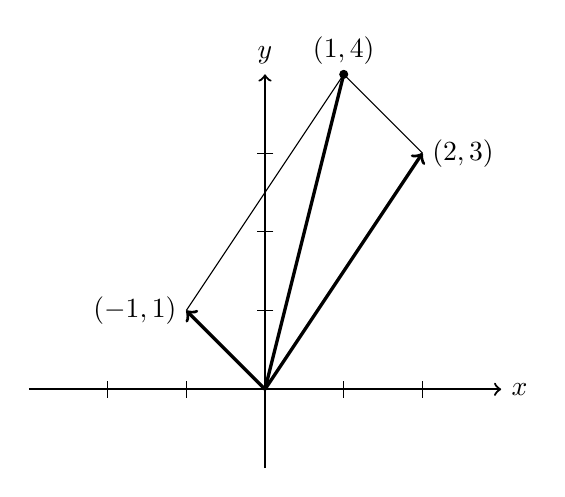
\begin{tikzpicture}[scale=1.0]
                \draw[thick,->] (-3.0,0) -- (3.0,0) node[right] {$x$}; % eje x
                \draw[thick,->] (0,-1) -- (0,4) node[above] {$y$}; % eje y
                \foreach \x in {-2,...,2}
                \draw (\x,3pt) -- (\x,-3pt);
                \foreach \y in {0,...,3}
                \draw (3pt,\y) -- (-3pt,\y) ;
                \draw[very thick, ->] (0,0) -- (-1,1);
                \node [left] at (-1,1) {$(-1,1)$};
                \draw[very thick,->] (0,0) -- (2,3);
                \node [right] at (2,3) {$(2,3)$};
                \draw[very thick,-] (0,0) -- (1,4);
                \node [above] at (1,4) {$(1,4)$};
                \draw[fill] (1,4) circle [radius=0.05];
                \draw[-] (-1,1) -- (1,4);
                \draw[-] (2,3) -- (1,4);
            \end{tikzpicture}
            \caption{Ejemplo de la ley del paralelogramo.}\label{fig-ley-del-paralelogramo}
        \end{figure} 
    \end{ejemplo*}
    
    \begin{ejemplo*}
        Sea $v= (3, 1)$ y $w=(1,2)$. Entonces
        \begin{equation*}
            v+w = (4,3). 
        \end{equation*}
        Esta suma la representamos en la fig. \ref{fig-ley-del-paralelogramo-2}. 
        \begin{figure}[h]
        	\centering
            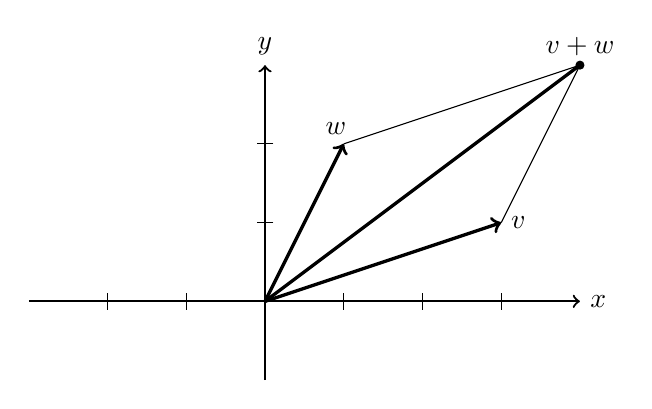
\begin{tikzpicture}[scale=1.0]
                \draw[thick,->] (-3.0,0) -- (4.0,0) node[right] {$x$}; % eje x
                \draw[thick,->] (0,-1) -- (0,3) node[above] {$y$}; % eje y
                \foreach \x in {-2,...,3}
                \draw (\x,3pt) -- (\x,-3pt);
                \foreach \y in {0,...,2}
                \draw (3pt,\y) -- (-3pt,\y) ;
                \draw[very thick, ->] (0,0) -- (3,1);
                \node [right] at (3,1) {$v$};
                \draw[very thick,->] (0,0) -- (1,2);
                \node [above] at (0.9,2) {$w$};
                \draw[very thick,-] (0,0) -- (4,3);
                \node [above] at (4,3) {$v+w$};
                \draw[fill] (4,3) circle [radius=0.05];
                \draw[-] (3,1) -- (4,3);
                \draw[-] (1,2) -- (4,3);
            \end{tikzpicture}
            \caption{La ley del paralelogramo.}\label{fig-ley-del-paralelogramo-2}
        \end{figure}
        
        Vemos de nuevo que en la representación geométrica aparece un paralelogramo. La razón por la cual la figura que aparece es un paralelogramo se puede dar en 	términos de la geometría plana de la siguiente manera. Obtenemos $v = (1, 2)$ comenzando desde el origen $0 = (0, 0)$, y moviéndonos 1 unidad hacia la derecha y 2 hacia arriba. Para obtener $v+w$, comenzamos desde $v$, y de nuevo nos movemos 1 unidad a la derecha y 2 hacia arriba. Así, el segmento entre 0 y $w$, y entre $v$ y $v+w$ son las hipotenusas de los triángulos rectángulos cuyos catetos  correspondientes son de la misma longitud y paralelos. Los segmentos anteriores son por lo tanto paralelos y de la misma longitud, como se ilustra en la fig. \ref{fig-ley-del-paralelogramo-3}. Esta forma geométrica de visualizar la suma de dos vectores en $\R^2$  es conocida como \textit{ley del parelogramo.}\index{ley del paralelogramos}
        \begin{figure}[h]
        	\centering
            \begin{tikzpicture}[scale=1.0]
            \draw[thick,->] (-3.0,0) -- (4.0,0) node[right] {$x$}; % eje x
            \draw[thick,->] (0,-1) -- (0,3) node[above] {$y$}; % eje y
            \foreach \x in {-2,...,3}
            \draw (\x,3pt) -- (\x,-3pt);
            \foreach \y in {0,...,2}
            \draw (3pt,\y) -- (-3pt,\y) ;
            \draw[very thick,-] (0,0) -- (1,2);
            \node [above] at (0.9,2) {$w$};
            \draw[very thick,-] (3,1) -- (4,3);
            \node [above] at (4,3) {$v+w$};
            \node [below] at (3,1) {$v$};
            \node [left] at (0,-0.3) {$0$};
            \draw [dashed] (1,0) -- (1,2);
            \draw [dashed] (3, 1) -- (4,1) -- (4,3);
            \draw[fill] (0,0) circle [radius=0.07];
            \draw[fill] (1,2) circle [radius=0.07];
            \draw[fill] (3,1) circle [radius=0.07];
            \draw[fill] (4,3) circle [radius=0.07];
            \end{tikzpicture}
            \caption{La ley del paralelogramo.}\label{fig-ley-del-paralelogramo-3}
        \end{figure}
    \end{ejemplo*}
    
    
    \begin{ejemplo*} Sea el punto $v =(3, 1)$ , entonces $-v = (- 3, - 1)$. Si dibujamos $v$ y $-v$ vemos que $-v$ es un vector del mismo ``tamaño'' que $v$ pero con la dirección opuesta. Podemos ver a $-v$ como la reflexión de $v$ a través del origen (fig. \ref{fig-vector-opuesto}). 
    \begin{figure}[h]
    	\centering
        \begin{tikzpicture}[scale=1.0]
        \draw[thick,->] (-4.0,0) -- (4.0,0) node[right] {$x$}; % eje x
        \draw[thick,->] (0,-2) -- (0,2) node[above] {$y$}; % eje y
        \foreach \x in {-3,...,3}
        \draw (\x,3pt) -- (\x,-3pt);
        \foreach \y in {-1,...,1}
        \draw (3pt,\y) -- (-3pt,\y) ;
        \draw[very thick, ->] (0,0) -- (3,1);
        \node [right] at (3,1) {$v$};
        \draw[very thick, ->] (0,0) -- (-3,-1);
        \node [left] at (-3,-1) {$-v$};
        \draw[fill] (0,0) circle [radius=0.1];
        \end{tikzpicture}
        \caption{El opuesto de un vector.}\label{fig-vector-opuesto}
    \end{figure}
    \end{ejemplo*}




    La resta de dos vectores también se puede representar geométricamente: restemos  al vector $v$ el vector $w$. Como primera opción podemos encontrar el  vector $-w$ y sumarlo  a $v$ aplicando la ley del paralelogramo. Esto es equivalente a lo siguiente: los vectores $v$ y $w$ determinan el triángulo determinado por los puntos $0$, $v$ y $w$. Entonces,  el lado determinado por $w$ y $v$,  en ese sentido, trasladado al origen es el vector $v-w$  (fig. \ref{fig-resta-de-vectores}). Claramente, esta forma geométrica de hacer la resta  es de nuevo una aplicación de la ley del paralelogramo, pues $(v-w)+ w= v$.
    \begin{figure}[h]
    	\centering
        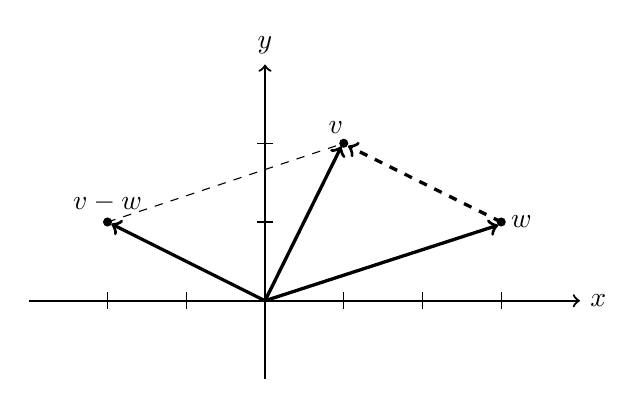
\begin{tikzpicture}[scale=1.0]
        \draw[thick,->] (-3.0,0) -- (4.0,0) node[right] {$x$}; % eje x
        \draw[thick,->] (0,-1) -- (0,3) node[above] {$y$}; % eje y
        \foreach \x in {-2,...,3}
        \draw (\x,3pt) -- (\x,-3pt);
        \foreach \y in {0,...,2}
        \draw (3pt,\y) -- (-3pt,\y) ;
        % vector w
        \draw[fill] (3,1) circle [radius=0.05];
        \node [right] at (3,1) {$w$};
        \draw[very thick, ->] (0,0) -- (2.96,0.96);
        % vector v
        \draw[fill] (1,2) circle [radius=0.05];
        \draw[very thick,->] (0,0) -- (0.97,1.96);
        \node [above] at (0.9,2) {$v$};
        % flecha punteada de w a v
        \draw[dashed,->,very thick] (3,1) -- (1.055,1.965);
        % vector v - w
        \draw[fill] (-2,1) circle [radius=0.05];
        \node [above] at (-2,1) {$v-w$};
        \draw[very thick,->] (0,0) -- (-2*0.975,1*0.975);	
        % punteada de v-w  a v
        \draw[dashed] (-2,1) -- (1,2);	
        \end{tikzpicture}
        \caption{Resta de vectores.}\label{fig-resta-de-vectores}
    \end{figure}
    
    

    Ahora consideraremos la multiplicación de un vector $v$ por un número. 
    
    \begin{definicion}\label{def-producto-escalar-x-rn}
        Sea $v = (x_1,\ldots,x_n) \in \R^n$ y $\lambda \in \R$, entonces
        \begin{equation*}
            \lambda.v = (\lambda x_1,\ldots,\lambda x_n).
        \end{equation*}  
        También denotamos a esta multiplicación por $\lambda v$.
    \end{definicion}

    \begin{ejemplo*}
         Si $v= (2, -1,5)$  y $\lambda = 7$, entonces $\lambda v = (14, -7.35)$.
    \end{ejemplo*}
    
    Es fácil verificar las siguientes reglas: dados $v,w \in \R^n$, 
    \begin{enumerate}
        \item[\textbf{P1.}] $1.v=v$.
        \item[\textbf{P2.}] $\lambda_1(\lambda_2v) = (\lambda_1\lambda_2)v$, para todo $\lambda_1,\lambda_2 \in \R$.
        \item[\textbf{D1.}] $\lambda(v+w) = \lambda v +\lambda w$, para todo $\lambda \in \R$  (\textit{propiedad distributiva}).
        \item[\textbf{D2.}] $(\lambda_1+\lambda_2)v = \lambda_1v + \lambda_2 v$ para todo $\lambda_1,\lambda_2 \in \R$  (\textit{propiedad distributiva}).
    \end{enumerate}

    También tengamos en cuenta que 
    \begin{equation*}
        (-1)v = -v.
    \end{equation*}
    
    ¿Cuál es la representación geométrica de la multiplicación de un vector  por un número?
    \begin{ejemplo*}
        Sea $v= (1,2)$ y $\lambda = 3$. Luego $\lambda v = (3,6)$ como en la siguiente figura:
        \begin{center}
            \begin{tabular}{ccc}
                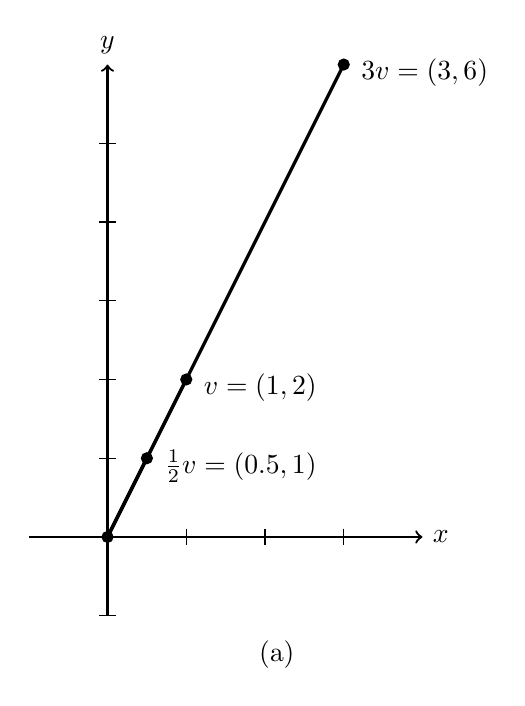
\begin{tikzpicture}[scale=1.0]
                \draw[thick,->] (-1.0,0) -- (4.0,0) node[right] {$x$}; % eje x
                \draw[thick,->] (0,-1) -- (0,6) node[above] {$y$}; % eje y
                \foreach \x in {0,...,3}
                \draw (\x,3pt) -- (\x,-3pt);
                \foreach \y in {-1,...,5}
                \draw (3pt,\y) -- (-3pt,\y) ;
                \draw[very thick, -] (0,0) -- (1,2);
                \node [right] at (1.1,1.9) {$v=(1,2)$};
                \draw[very thick, -] (0,0) -- (3,6);
                \node [right] at (3.1,5.9) {$3v=(3,6)$};
                \draw[very thick, -] (0,0) -- (0.5,1);
                \node [right] at (0.6,0.9) {$\frac12v=(0. 5,1)$};
                \draw[fill] (0,0) circle [radius=0.07];
                \draw[fill] (0.5,1) circle [radius=0.07];
                \draw[fill] (3,6) circle [radius=0.07];
                \draw[fill] (1,2) circle [radius=0.07];
                \node [right] at (1.8,-1.5) {(a)};
                \end{tikzpicture}
                &\qquad &
                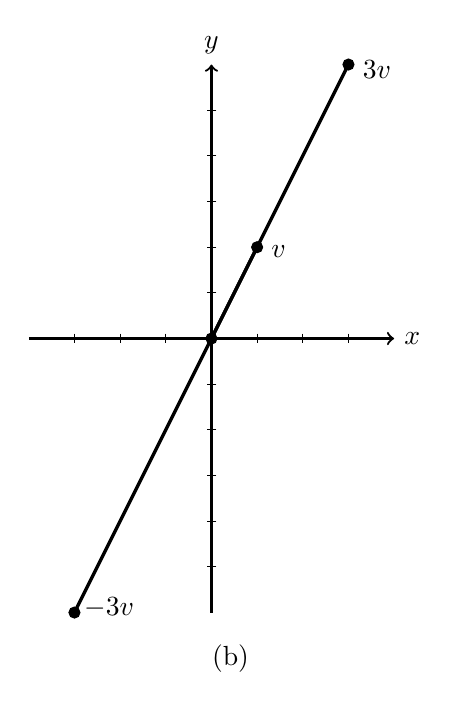
\begin{tikzpicture}[scale=0.58]
                \draw[thick,->] (-4.0,0) -- (4.0,0) node[right] {$x$}; % eje x
                \draw[thick,->] (0,-6) -- (0,6) node[above] {$y$}; % eje y
                \foreach \x in {-3,...,3}
                \draw (\x,3pt) -- (\x,-3pt);
                \foreach \y in {-5,...,5}
                \draw (3pt,\y) -- (-3pt,\y) ;
                \draw[very thick, -] (0,0) -- (1,2);
                \node [right] at (1.1,1.9) {$v$};
                \draw[very thick, -] (0,0) -- (3,6);
                \node [right] at (3.1,5.9) {$3v$};
                \draw[very thick, -] (0,0) -- (-3,-6);
                \node [right] at (-3.0,-5.9) {$-3v$};
                \draw[fill] (0,0) circle [radius=0.12];
                \draw[fill] (-3,-6) circle [radius=0.12];
                \draw[fill] (3,6) circle [radius=0.12];
                \draw[fill] (1,2) circle [radius=0.12];
                \node [right] at (-0.2,-7) {(b)};
                \end{tikzpicture}
            \end{tabular}
        \end{center}
            
            
    \end{ejemplo*}

     La multiplicación por 3 equivale a ``estirar'' $v$ por 3. Del mismo modo, $\frac12v$ 	equivale a estirar $v$ en $\frac12$, es decir, reducir $v$ a la mitad de su tamaño. En general, si $t$ es un número con $t> 0$, interpretamos $tv$ como un punto en la misma dirección que $v$ con tamaño  $t$-veces el tamaño de $v$.  De hecho, decimos que $v$ y $w$ tienen la misma dirección si existe un número $\lambda> 0$ tal que $v = \lambda w$. La multiplicación por un número negativo invierte la dirección. Así, $-3 v$ se representa como en la figura anterior, en la parte (b). Decimos que $v$ y $w$  (ninguno de los cuales es cero) tienen direcciones opuestas si existe un número $\lambda <0$ tal que $v =\lambda w$. Por lo tanto, $-v$ tiene dirección opuesta a $v$.

        
Más allá de las interpretaciones geométricas,  hemos definido  en forma algebraica la suma de vectores en $\R^n$ y  la multiplicación de un vector por un escalar,  y estas operaciones tienen ciertas propiedades de interés. 

Concluyendo, las definiciones y resultados más importantes de esta sección son:


Sean  $(x_1,\ldots,x_n), (y_1,\ldots,y_n) \in \R^n$ y $\lambda \in \R$, definimos
    \begin{itemize}
        \item $(x_1,\ldots,x_n)+ (y_1,\ldots,y_n):=(x_1+y_1,\ldots,x_n+y_n)$, 
        \item $\lambda.v := (\lambda x_1,\ldots,\lambda x_n)$.
    \end{itemize}
Dados  $v,w,u$ en $\R^n$,  se verifican

    \begin{enumerate}
        \item[\textbf{S1.}] $v + w = w + v$ (\textit{conmutatividad de la suma}),
        \item[\textbf{S2.}] $(v+ w)+ u = v + (w+u)$ (\textit{asociatividad de la suma}),
        \item[\textbf{S3.}] sea $0: =(0,\ldots, 0)$, el \textit{vector cero}, entonces $0+ v = v + 0 =v$ (\textit{existencia de elemento neutro de la suma}).
        \item[\textbf{S4.}] Si $v =(x_1,\ldots,x_n)$, entonces $-v:=(-x_1,\ldots,-x_n)$ y se satisface  $v + (-v) = (-v)+ v =0$ (\textit{existencia de opuesto} o  \textit{inverso aditivo}).
        \item[\textbf{P1.}] $1.v=v$.
        \item[\textbf{P2.}] $\lambda_1(\lambda_2v) = (\lambda_1\lambda_2)v$, para todo $\lambda_1,\lambda_2 \in \R$.
        \item[\textbf{D1.}] $\lambda(v+w) = \lambda v +\lambda w$, para todo $\lambda \in \R$  (\textit{propiedad distributiva}).
        \item[\textbf{D2.}] $(\lambda_1+\lambda_2)v = \lambda_1v + \lambda_2 v$ para todo $\lambda_1,\lambda_2 \in \R$  (\textit{propiedad distributiva}).
    \end{enumerate}





Verán más adelante que las propiedades anteriores son muy parecidas a los  ``axiomas'' que se utilizan en el  capítulo \ref{chap-esp-vect} para definir espacios vectoriales abstractos (ver definición \ref{def-esp-vect}). 



    \begin{definicion}\label{def-base-canonica-rn}
    Dado, $n \in \mathbb N$, para cada $i\in\{1, ..., n\}$, se denota ${e_i}\in\R^n$ al vector cuyas coordenadas son todas $0$ excepto la coordenada $i$ que es un $1$.
    \begin{align*}
    e_i:=(0, ..., 1, ..., 0)
    \end{align*}
    El conjunto $\{e_1, ..., e_n\}$ se llama\textit{ {base canónica}} de $\R^n$.\index{base canónica}
\end{definicion}

\begin{ejemplo*}
    En $\R^3$ los vectores son $
    e_1=(1,0,0)$, $
    e_2=(0,1,0)$, 
    $e_3=(0,0,1)
    $
\end{ejemplo*}

Estos vectores jugarán un rol central en la materia, principalmente, por la siguiente propiedad.


\begin{proposicion}
    Todo vector de $\R^n$ se escribe como combinación lineal de la base canónica. Explícitamente, si $(x_1, ..., x_n)\in\R^n$ entonces
    \begin{align*}
    (x_1, ..., x_n)=x_1e_1+x_2e_2+\cdots+x_ne_n.
    \end{align*}
\end{proposicion}


La demostración es trivial pero por ahora no la haremos. 


\begin{ejemplo*}
    
    \begin{align*}
    (1,2,3)&=(1,0,0)+(0,2,0)+(0,0,3)\\
    &=1(1,0,0)+2(0,1,0)+3(0,0,1)\\
    &=1e_1+2e_2+3e_3
    \end{align*}
    
\end{ejemplo*}




\subsection*{$\S$ Ejercicios}   
\begin{enumex}
    \item Dados $v = (-1, 2-0)$, $w = (2,-3,-1)$ y $u = (1,-1,1)$, calcular:
    \begin{enumex}
    % 	\item $v + w$, 
    % 	\item $v - w$, 
        \item $2v + 3w -5u$,
        \item $5(v+w)$, 
        \item $5v + 5w$ (y verificar que es igual al vector de arriba).
    \end{enumex}
\end{enumex}




\end{section}
    
    
    
    \begin{section}{El producto escalar}\label{seccion-el-producto-escalar}
        
        En 2-espacios, dados dos vectores $v = (x_1, x_2)$ y $w= (y_l, y_2)$, definimos su \textit{producto escalar}\index{producto escalar} como
        \begin{equation*}
            \langle v , w  \rangle :=x_1y_1 + x_2y_2.
        \end{equation*}
        Para el caso de 3-espacios, sean   $v = (x_1, x_2,x_3)$ y $w= (y_l, y_2,y_3)$,  entonces el \textit{producto escalar de $v$ y $w$} es
        \begin{equation*}
            \langle v , w  \rangle :=x_1y_1 + x_2y_2+x_3y_3.
        \end{equation*}
        Finalmente, en los $n$-espacios,  generalizamos la definición de la manera obvia: 
        
        \begin{definicion}
            Sean  $v = (x_1, \ldots,x_n)$ y $w= (y_l, \ldots,y_n)$ vectores de $\R^n$,  el \textit{producto escalar de $v$ y $w$}\index{producto escalar} se define como		
            \begin{equation*}
            \langle v , w \rangle :=x_1y_1 + x_2y_2+\cdots+x_ny_n.
            \end{equation*}
        \end{definicion}
        
        
        
        Es importante notar  que este producto es un número real. Por ejemplo, si
        \begin{equation*}
            v= (1, 3, - 2) \quad\text{ y } \quad w= (- 1, 4, - 3),
        \end{equation*}
        entonces
        \begin{equation*}
            \langle v , w \rangle= - 1 + 12 + 6 = 17.
        \end{equation*}
        
        Por el momento, no le damos una interpretación geométrica a este producto escalar y veremos esto en la sección \ref{secccion-norma-de-un-vector}. Ahora derivaremos algunas propiedades importantes.
        
        \begin{proposicion}\label{propiedades-del-producto-escalar}
           Sean $v$, $w$, $u$  tres vectores en $\R^n$, entonces
     
        \begin{enumerate}[label=\textbf{P\arabic*.},ref=P\arabic*]
            \item\label{prop-P1}	$\langle v , w \rangle = \langle w , v \rangle$.
            \item\label{prop-P2} 
            \begin{equation*}
                \langle v , w + u \rangle =\langle v , w \rangle + \langle v , u \rangle = \langle w +u , v \rangle.
            \end{equation*}
            \item\label{prop-P3} Si $\lambda$ es un número, entonces 
            \begin{equation*}
                \langle \lambda v , w \rangle = \lambda \langle v , w \rangle \quad \text{ y } \quad  \langle v , \lambda w \rangle = \lambda \langle v , w \rangle.
            \end{equation*}
            \item\label{prop-P4} Si $v=0$ es el vector cero, entonces $\langle v , v \rangle =0$,  de lo contrario
            \begin{equation*}
                \langle v , v \rangle >0
            \end{equation*}
        \end{enumerate}
        \end{proposicion}
        \begin{proof} Expresemos los tres vectores en coordenadas:  $v = (x_1, \ldots,x_n)$, $w =  (y_1, \ldots, y_n)$, $u = (z_1, \ldots, z_n)$. 

            \ref{prop-P1}.
        \begin{equation*}
            x_1y_1 + x_2y_2+\cdots+x_ny_n = y_1x_1 + y_2x_2+\cdots+y_nx_n
        \end{equation*}
        porque para cualquiera de los dos números $x, y$, tenemos que $xy=yx$. Esto prueba la propiedad . 
        
        Para \ref{prop-P2}, sea $u = (z_1, \ldots, z_n)$. Entonces
        \begin{equation*}
            w + u = (y_1+z_1, \ldots, y_n+ z_n)
        \end{equation*}
        y
        \begin{align*}
            \langle v , w + u \rangle &= \langle (x_1, \ldots,x_n) , (y_1+z_1, \ldots, y_n+ z_n) \rangle\\
            &= x_1(y_1+z_1) + \cdots x_n(y_n+z_n) \\
            &= x_1y_1+x_1z_1 + \cdots x_ny_n+x_nz_n
        \end{align*}
        Reordenando los términos obtenemos
        \begin{equation*}
                \langle v , w + u \rangle =  x_1y_1+\cdots +  x_ny_n +x_1z_1 + \cdots+x_nz_n,
        \end{equation*}
        que no es otra cosa que $\langle v , w \rangle + \langle v , u \rangle$.
        
        Dejamos la propiedad \ref{prop-P3} como ejercicio.
        
        Finalmente probemos \ref{prop-P4}. Observemos que 
        \begin{equation}\label{eq-v-escalar-v}
            \langle v , v \rangle = x_1^2 + x_2^2 + \cdots + x_n^2.
        \end{equation}
        Como $x_i^2 \ge 0$ para todo $i$,  entonces $\langle v , v \rangle \ge 0$. Además, es claro que si $v$ tiene todas las coordenadas iguales a 0,  entonces  $\langle v , v \rangle =0$. En  el caso que $v\not=0$, entonces,  existe algún $i$  tal que  $x_i \ne 0$, por lo tanto $x_i^2>0$ y por la ecuación \eqref{eq-v-escalar-v}, tenemos que  $\langle v , v \rangle>0$.
    \end{proof}

        Por  la propiedad \ref{prop-P1} diremos que el producto escalar es \textit{simétrico}, por las propiedades  \ref{prop-P2} y \ref{prop-P3} diremos que es una \textit{forma bilineal} y, finalmente, por la propiedad \ref{prop-P4} diremos que es \textit{definido positivo.} 
        
        El producto escalar $\langle v , w \rangle$ puede ser  igual a 0 para determinados  vectores,  incluso ambos distintos de 0.  Por ejemplo, si $v = (1,2,3)$ y $w = (2, 1, -\frac43)$,  entonces
        \begin{equation*}
            \langle v , w \rangle = 2 + 2 -4 =0.
        \end{equation*}
        \begin{definicion}
            Decimos que dos vectores $v$ y $w$ en $\mathbb R^n$ son  \textit{perpendiculares} u \textit{ortogonales}\index{vectores ortogonales}\index{vectores perpendiculares} si  $\langle v , w \rangle=0$. Cuando $v$ y $w$ son ortogonales  denotamos $v \perp w$.
        \end{definicion}
        
        Por el momento, no es claro que en el plano la definición anterior coincida con nuestra noción geométrica e intuitiva de perpendicularidad. Esto lo veremos en la siguiente sección. Aquí nos limitaremos a observar un ejemplo.
        
        \begin{ejemplo*}
            En  $\R^3$ consideremos los vectores
            \begin{equation*}
            e_1 = (1,0,0),\quad e_2 = (0, 1,0),\quad e_3 = (0,0,1),
            \end{equation*}
            representados en la fig. \ref{fig-canonicos-en-R3}
            \begin{figure}[h]
            	\centering
                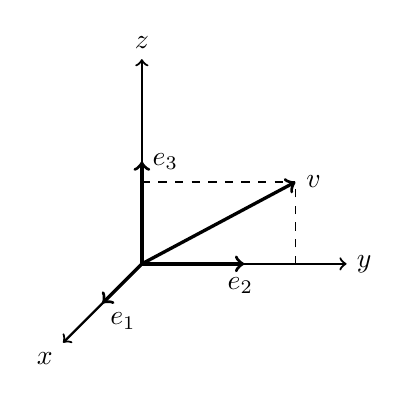
\begin{tikzpicture}[scale=1.3]
                %draw the main coordinate system axes
                \draw[thick,->] (0,0,0) -- (2,0,0) node[right]{$y$};
                \draw[thick,->] (0,0,0) -- (0,2,0) node[above]{$z$};
                \draw[thick,->] (0,0,0) -- (0,0,2) node[anchor=north east]{$x$};
                \draw[very thick,->] (0,0,0) -- (1,0,0);
                \node [below] at (1,0,0.1) {$e_2$};
                \draw[very thick,->] (0,0,0) -- (0,1,0) node[anchor=west]{$e_3$};
                \draw[very thick,->] (0,0,0) -- (0,0,1);
                \node [below] at (0.2,0,1) {$e_1$};
                \draw [dashed] (0,0.8,0) -- (1.5,0.8,0);
                \draw [dashed] (1.5,0,0) -- (1.5,0.8,0);
                \draw[very thick,->] (0,0,0) -- (1.5,0.8,0) node[right]{$v$};
                \end{tikzpicture}
                \caption{Vectores canónicos en $\R^3$.}
                \label{fig-canonicos-en-R3}
            \end{figure}
            
            Luego, vemos que $\langle e_i , e_j \rangle = 0$, si $i \ne j$ y por lo tanto $e_i$  es perpendicular a $e_j$ si $i \ne j$, lo cual concuerda con nuestra intuición. 
        \end{ejemplo*} 
            
            Observemos que si $v = (x_1,x_2,x_3)$,  entonces $\langle v , e_i \rangle = x_i$. Por lo tanto,  si la coordenada $i$-ésima de $v$ es cero,  $v$  es ortogonal a $e_i$. Esto nos dice,  por ejemplo,  que si $v$  es un vector contenido en el plano que incluye $e_2$ y $e_3$,  es decir si la primera coordenada es cero,  entonces $v$  es ortogonal a $e_1$. 
            
        
        \begin{ejemplo*} Sea $(a,b)$ un vector en $\R^2$, entonces $(-b,a)$ es un vector ortogonal a $(a,b)$ debido a que
            \begin{equation*}
                \langle (a,b) , (-b,a) \rangle = a\cdot b + (-b) \cdot a = 0.
            \end{equation*}
            Si graficamos con un ejemplo, $a=1$, $b=3$; vemos que esto se corresponde con nuestra intuición de perpendicularidad. 
                
            \begin{center}
                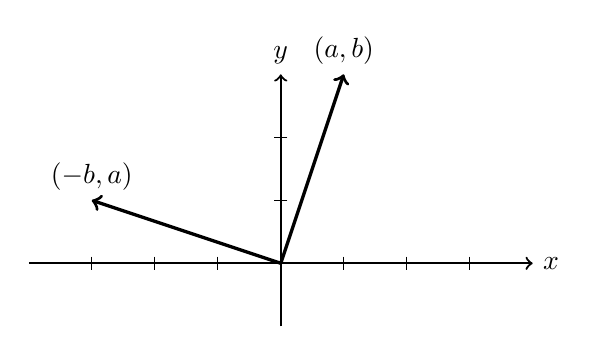
\begin{tikzpicture}[scale=0.8]
                \draw[thick,->] (-4.0,0) -- (4.0,0) node[right] {$x$}; % eje x
                \draw[thick,->] (0,-1) -- (0,3) node[above] {$y$}; % eje y
                \foreach \x in {-3,...,3}
                \draw (\x,3pt) -- (\x,-3pt);
                \foreach \y in {0,...,2}
                \draw (3pt,\y) -- (-3pt,\y) ;
                % vector w
                \draw[very thick,->] (0,0) -- (1,3);
                \node [above] at (1,3) {$(a,b)$};
                \draw[very thick,->] (0,0) -- (-3,1);
                \node [above] at (-3,1) {$(-b,a)$};
                \end{tikzpicture}
            \end{center}	
                
        \end{ejemplo*}
        

        \subsection*{$\S$ Ejercicios}
        \begin{enumex}
            
            \item Calcular los siguientes productos escalares. %\langle v , w  \rangle
            \begin{enumex}
              \item $\langle (-1, 2-0) ,(2,-3,-1) \rangle$, 
            %   \item  $\langle (2,4,-3,-1),(1,-1,2, 1) \rangle$,
              \item  $\langle (4,-1),(-1,2) \rangle$.
            \end{enumex}
            
            \vskip .2cm
            
            \item Dados $v = (-1, 2-0)$, $w = (2,-3,-1)$  y $u = (1,-1,1)$, verificar que:
            \begin{equation*}
                \langle 2v + 3w , -u   \rangle = -2\langle v ,u \rangle -3 \langle w , u  \rangle
            \end{equation*}
            
            \vskip .2cm
        
            \item Sea $v=(x_1,x_2,x_3)\in\R^3$ y sea $e_1$, $e_2$ y $e_3$ la base canónica de $\R^3$ (ver definición \ref{def-base-canonica-rn}). Verificar que 
            $$v=x_1e_1+x_2e_2+x_3e_3=\langle v,e_1\rangle e_1+\langle v,e_2\rangle e_2+\langle v,e_3\rangle e_3.$$
    \vskip .2cm
    
    \item Probar, usando sólo las propiedades \textbf{P1}, \textbf{P2}, y \textbf{P3} del producto escalar, que dados $v, w, u \in \mathbb R^n$ y $\lambda_1, \lambda_2 \in \mathbb R$, 
    \begin{enumex}
        \item se cumple:
        \begin{equation*}
        \langle \lambda_1 v + \lambda_2 w , u  \rangle =  \lambda_1\langle v , u  \rangle +   \lambda_2\langle w , u  \rangle.
        \end{equation*}
        \item Si $\langle v , w  \rangle =0$, es decir si $v$ y $w$ son ortogonales,  entonces
        \begin{equation*}
            \langle \lambda_1 v + \lambda_2 w ,  \lambda_1 v + \lambda_2 w   \rangle =
            \lambda_1^2 \langle  v ,  v  \rangle + \lambda_2^2 \langle w,w  \rangle.
        \end{equation*}
    \end{enumex}
    
    \vskip .2cm
                
    \item Probar  que 
    \begin{enumex}
        \item $(2,3,-1)$ y $(1, -2, -4)$ son ortogonales.
        \item $(2,-1)$ y $(1,2)$ son ortogonales. Dibujar en el plano. 
    \end{enumex}
    \vskip .2cm
    \item Encontrar 
        \begin{enumex}
            \item un vector no nulo ortogonal  a $(3,-4)$,
            \item un vector no nulo ortogonal a $(2,-1,4)$,
            \item un vector no nulo ortogonal a $(2,-1,4)$ y $(0,1,-1)$,
        \end{enumex}
    \end{enumex}

    \end{section}

    \begin{section}{La norma de un vector}\label{secccion-norma-de-un-vector}
    Si $v$  es vector,  entonces $\langle v , v \rangle \ge 0$ y definimos como la \textit{norma de $v$}\index{norma de un vector} o \textit{longitud de $v$} al número
    \begin{equation*}
        ||v|| = \sqrt{\langle v , v \rangle}.
    \end{equation*}
    
    Cuando $v$ pertenece al plano  y $v =(x,y)$,  entonces $||v|| = \sqrt{x^2 + y^2}$ y si graficamos el vector en la fig. \ref{fig-pitagoras}, vemos que la noción de norma o longitud en $\R^2$ se deduce del teorema de Pitágoras.  
    \begin{figure}[h]
    	\centering
        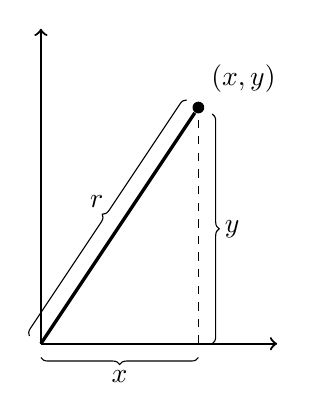
\begin{tikzpicture}
        \draw[thick,->] (0,0) coordinate (O) -- (3,0);
        \draw[thick,->] (O) -- (0,4);
        \node[inner sep=1.5pt,fill,circle,label={60:$(x,y)$}] at (2,3) (point) {};
        \draw[very thick] (0,0) -- (point);
        %\draw (1.8,0) -- ++(0,0.2) -- ++(0.2,0);
        \draw[dashed] (2,0) coordinate (pointx) -- (point); 
        \draw[decoration={brace,mirror,raise=5pt},decorate]
        (2,0) -- node[right=6pt] {$y$} (point);
        \draw[decoration={brace,mirror,raise=5pt},decorate]
        (0,0) -- node[below=6pt] {$x$} (2,0); 
        \draw[decoration={brace,raise=5pt},decorate]
        (0,0) -- node[below=6pt] {${}$} (2,3);
        \node [right] at (0.5,1.8) {$r$};
        \end{tikzpicture}
        \caption{$r= \sqrt{x^2 + y^2}$.}
        \label{fig-pitagoras}
    \end{figure} 

    Si $n=3$,  el dibujo es como en la fig. \ref{fig-pitagoras-3d}, para $v =(x,y,z)$.  Es decir,  por la aplicación reiterada del teorema de Pitágoras obtenemos que la longitud de $v$ es $\sqrt{x^2 + y^2 +z^2}$.
    \begin{figure}[h]
    	\centering
        \begin{tikzpicture}[scale=0.8]
        \draw[thick,->] (0,0,0) -- (5,0,0) node[right]{$y$};
        \draw[thick,->] (0,0,0) -- (0,5,0) node[above]{$z$};
        \draw[thick,->] (0,0,0) -- (0,0,5) node[anchor=north east]{$x$};
        \draw[very thick,->] (0,0,0) -- (4,4.5,3) node[anchor=west]{$v$};
        \draw[dashed]  (0,0,0) -- (4,0,3); 
        \draw[dashed]  (0,0,3) -- (4,0,3); 
        \draw[dashed]  (4,0,0) -- (4,0,3); 
        \draw[dashed]  (4,0,3) -- (4,4.5,3); 
        %\draw[decoration={brace,raise=5pt},decorate]
        %(0,0,0) -- node[below=6pt] {${}$} (4,4.5,3);
        \node [right] at (2,2.2,1.5) {$r$};
        \node [right] at (1.2,-0.1,1.5) {$w$};
        \node [below] at (4.2,0.2,3.5) {$(x,y)$};
        \end{tikzpicture}
        \caption{$w= \sqrt{x^2 + y^2}$, $r = \sqrt{w^2 + z^2} = \sqrt{x^2 + y^2 +z^2}$.}
        \label{fig-pitagoras-3d}
    \end{figure} 
    
    En  general,  si $v =(x_1,x_2,\ldots,x_n) \in \R^n$,  entonces
    \begin{equation*}
        ||v|| = \sqrt{x_1^2+x_2^2+\cdots+x_n^2}
    \end{equation*} 
    y la aplicación reiterada del  teorema de Pitágoras nos dice que esta es la definición correcta de longitud o norma de un vector. 
    
    \begin{proposicion}\label{prop-lambda-norma}
        Sea $v \in \R^n$ y $\lambda \in \R$,  entonces
        \begin{equation*}
            ||\lambda v|| = |\lambda|||v||.
        \end{equation*}
    \end{proposicion}
    \begin{proof}
        $||\lambda v||^2 = \la\lambda v, \lambda v \ra$, por la propiedad \ref{prop-P3} del producto escalar, 
        \begin{equation*}
            \la\lambda v, \lambda v \ra = \lambda\la v, \lambda v \ra = \lambda^2\la v, v  \ra.
        \end{equation*}
        Es decir 	$||\lambda v||^2 =  \lambda^2 ||v||^2$, por lo tanto (sacando raíz cuadrada), $||\lambda v|| = |\lambda|||v||$.
    \end{proof}
    
El producto escalar no sólo es útil para definir la longitud de un vector,  sino que también nos dice cual es el ángulo entre dos vectores: sean   $v_1= (x_1,y_1)$ y $v_2= (x_2,y_2)$ en $\R^2$; veremos a continuación que 
        \begin{equation}\label{eq-cos-theta}
        \langle v_1 , v_2 \rangle = ||v_1||\, ||v_2|| \cos(\theta),
        \end{equation}
        donde  $\theta$ es el ángulo comprendido entre $v_1$ y $v_2$.
    
        
        Sea $\alpha_1$ el ángulo comprendido  entre $v_1$ y el eje horizontal y $\alpha_2$ el ángulo comprendido  entre $v_2$ y el eje horizontal.  Entonces,
        \begin{equation*}
        v_1 = ||v_1||(\cos (\alpha_1), \sen(\alpha_1) ), \quad v_2 = ||v_2||(\cos (\alpha_2), \sen(\alpha_2) ),
        \end{equation*}
        por lo tanto
        \begin{equation*}
        \langle v_1 , v_2 \rangle =  ||v_1|| \,  ||v_2|| (\cos (\alpha_1)\cos(\alpha_2)+  \sen(\alpha_1)\sen\alpha_2)). 
        \end{equation*}
        Por otro  lado, por la propiedad de la suma de los cosenos tenemos que 
        \begin{equation}\label{eq-ley-cosenos}
        \cos (\alpha_1)\cos(\alpha_2)+  \sen(\alpha_1)\sen(\alpha_2) = \cos(\alpha_1- \alpha_2).
        \end{equation}
        Es decir, 
        \begin{equation}
        \langle v_1,v_2 \rangle =   ||v_1|| \,  ||v_2|| \cos (\alpha_1-\alpha_2), 
        \end{equation}
        y precisamente, $\theta =  \alpha_1-\alpha_2$ es el ángulo comprendido entre  $v_1$ y $v_2$.
        
        Esto se puede generalizar a $\R^3$  y ahí en vez de la fórmula \eqref{eq-ley-cosenos} se debe usar la ley esférica de los cosenos. Los resultados se puede generalizar a  $\R^n$ y  en general vale  que si $v_1, v_2 \in \R^n$,  entonces el ángulo comprendido entre $v_1$ y $v_2$ es 
        \begin{equation}\label{eq-ang-comprendido}
        \theta = 	\operatorname{arcos}\left(\frac{\langle v_1 , v_2 \rangle}{||v_1|| \,  ||v_2|| }\right).
        \end{equation}  
        
 


        Terminaremos esta sección dando la noción de  distancia entre dos vectores o dos puntos. 
        
        \begin{definicion}
            Sea $v,w \in \R^n$, entonce las \textit{distancia}\index{distancia en $\mathbb R^n$} entre $v$ y $w$ es $||v-w||$.
        \end{definicion}
    
    Vemos en la fig. \ref{fig-distancia-de-vectores} que la norma del vector $v-w$ es la longitud del segmento que une $w$ con $v$.

\begin{figure}[h]
	\centering
    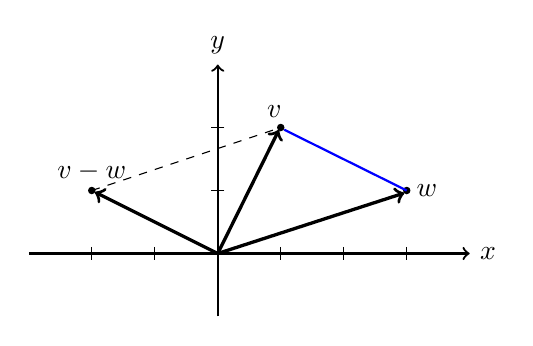
\begin{tikzpicture}[scale=0.8]
    \draw[thick,->] (-3.0,0) -- (4.0,0) node[right] {$x$}; % eje x
    \draw[thick,->] (0,-1) -- (0,3) node[above] {$y$}; % eje y
    \foreach \x in {-2,...,3}
    \draw (\x,3pt) -- (\x,-3pt);
    \foreach \y in {0,...,2}
    \draw (3pt,\y) -- (-3pt,\y) ;
    % vector w
    \draw[fill] (3,1) circle [radius=0.05];
    \node [right] at (3,1) {$w$};
    \draw[very thick, ->] (0,0) -- (2.96,0.96);
    % vector v
    \draw[fill] (1,2) circle [radius=0.05];
    \draw[very thick,->] (0,0) -- (0.97,1.96);
    \node [above] at (0.9,2) {$v$};
    % flecha punteada de w a v
    \draw[-, thick,blue] (3,1) -- (1.055,1.965);
    % vector v - w
    \draw[fill] (-2,1) circle [radius=0.05];
    \node [above] at (-2,1) {$v-w$};
    \draw[very thick,->] (0,0) -- (-2*0.975,1*0.975);	
    % punteada de v-w  a v
    \draw[dashed] (-2,1) -- (1,2);	
    \end{tikzpicture}
    \caption{Distancia de $v$ a $w$.}\label{fig-distancia-de-vectores}
\end{figure}


Una de las desigualdades más notables referentes a la norma de un vector es la \textit{desigualdad triangular}:\index{desigualdad triangular}

\begin{proposicion}
    Sean $v, w \in \R^n$, entonces
    \begin{equation*}
        ||v+w|| \le ||v||+||w||,
    \end{equation*}
    y la igualdad se cumple sólo cuando $w$ es múltiplo de $v$. 
\end{proposicion}
\begin{proof}[Demostración] Podemos probar  este resultado en base a una demostración ``geométrica'' basada en el hecho de que $|\cos\theta| \le 1 $ y luego utilizando la ecuación $\ref{eq-cos-theta}$. Más formalmente en el capítulo  \ref{chap-esp-prod-int} se verá que 
$$
\langle v_1,v_2 \rangle  \le   ||v_1|| \,  ||v_2||
$$
(proposición \ref{prop-cauchy-schwarz}, desigualdad de Cauchy-Schwarz) y de esta desigualdad se deduce fácilmente la desigualdad triangular probando que
$$
||v+w||^2 \le (||v||+||w||)^2.
$$
\begin{comment}
   Sea $v= (x_1,\ldots,x_n)$ y $w = (y_1,,\ldots,y_n)$. Luego $v+w = (x_1+ y_1,\ldots, x_n + y_n)$. Debemos probar entonces que
    \begin{equation*}
    \sqrt{\sum (x_i+ y_i)^2} \le  \sqrt{\sum x_i^2} + \sqrt{\sum y_i^2},
    \end{equation*}
    (todas las sumatoria sobre $i$). Si elevamos al cuadrado obtenemos:
    \begin{align*}
        \sum (x_i+ y_i)^2 &\le\sum x_i^2  + \sum y_i^2+ 2\sqrt{\sum x_i^2}\sqrt{\sum y_i^2}\\
        &\Updownarrow\\
        \sum  x_i^2+ y_i^2 + 2x_iy_i &\le \sum  x_i^2+ y_i^2 + 2\sqrt{\sum x_i^2}\sqrt{\sum y_i^2}\\
        &\Updownarrow\\
        \sum x_iy_i &\le \sqrt{\sum x_i^2}\sqrt{\sum y_i^2}.
    \end{align*}
    Si elevamos al cuadrado de nuevo obtenemos que
    \begin{equation*}
        ||v+w|| \le ||v||+||w|| \quad \Leftrightarrow \quad   (\sum x_iy_i)^2 \le \sum x_i^2\sum y_i^2.
    \end{equation*}

    Ahora bien
    \begin{align*}
        (\sum_i x_iy_i)^2  &= \sum_{i,j} x_iy_ix_jy_j \\
        &= \sum_i   x_iy_i x_iy_i + \sum_{i \ne j}  x_iy_ix_jy_j \\
        &= \sum_i   x_i^2y_i^2  +2 \sum_{i < j}  x_iy_ix_jy_j
    \end{align*}
\end{comment} 
\end{proof}

La desigualdad triangular expresa en forma algebraica el resultado, más conocido, ``en todo triángulo, un lado es menor que la suma de los otros dos'', que graficamos a continuación.

\begin{center}
        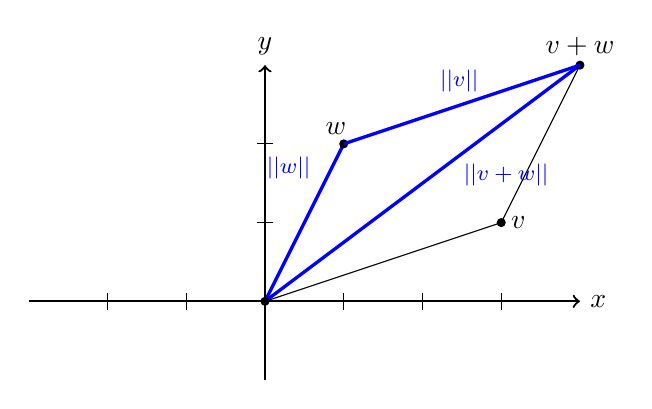
\begin{tikzpicture}[scale=1.0]
        \draw[thick,->] (-3.0,0) -- (4.0,0) node[right] {$x$}; % eje x
        \draw[thick,->] (0,-1) -- (0,3) node[above] {$y$}; % eje y
        \foreach \x in {-2,...,3}
        \draw (\x,3pt) -- (\x,-3pt);
        \foreach \y in {0,...,2}
        \draw (3pt,\y) -- (-3pt,\y) ;
        \draw[-] (0,0) -- (3,1);
        \node [right] at (3,1) {$v$};
        \draw[very thick,-,blue] (0,0) -- (1,2);
        \node [above] at (0.9,2) {$w$};
        \draw[very thick,-,blue] (0,0) -- (4,3);
        \node [above] at (4,3) {$v+w$};
        \draw[fill] (4,3) circle [radius=0.05];
        \draw[fill] (1,2) circle [radius=0.05];
        \draw[fill] (3,1) circle [radius=0.05];
        \draw[fill] (0,0) circle [radius=0.05];
        \draw[-] (3,1) -- (4,3);
        \draw[very thick,-,blue] (1,2) -- (4,3);
        \node [right,blue] at (-0.1,1.7) {{\footnotesize$||w||$}};
        \node [right,blue] at (2.4,1.6) {{\footnotesize$||v+w||$}};
        \node [right, blue] at (2.1,2.8) {{\footnotesize$||v||$}};
        \end{tikzpicture}
\end{center}
    




    \subsection*{$\S$ Ejercicios}

\begin{enumex}


    \item Encontrar la longitud de los vectores.
    \begin{align*}
    &(a) \ (2,3), && (b) \ (t,t^2), & (c) \ (\cos\phi,\sen\phi).
    \end{align*}
    
    \vskip .2cm
    
    \item Calcular $\langle v , w  \rangle$ y el {á}ngulo entre $v$ y $w$  para los siguientes vectores.
    \begin{align*}
    &(a) \ v=(2,2), w=(1,0), &&  (b) \  v=(-5,3,1), w=(2,-4,-7).
    \end{align*}
    
    \vskip .2cm
 
    
    
    \item Dados $v, w,\in \mathbb R^n$, probar que si  $\langle v , w  \rangle =0$, es decir si $v$ y $w$ son ortogonales,  entonces
        \begin{equation*}
        ||v + w||^2 = ||v||^2 + ||w||^2.
        \end{equation*}
        ¿Cuál es el nombre con que se conoce este resultado en $\mathbb R^2$?
        
    
        \vskip .2cm
     
    \item Sean $v,w\in \mathbb R^2$, probar usando  solo la definición explícita del producto escalar en $\mathbb R^2$ que 
    \begin{equation*}
        |\langle v , w  \rangle| \le ||v||\,||w|| \qquad \text{(Desigualdad de Cauchy-Schwarz).}
    \end{equation*}
    [Ayuda: elevar al cuadrado y aplicar la definición.]
   
    \item\label{ejercicio-identidad-de-polarizacion} (\textsc{Identidad de polarización}) Probar que 
    $$
    \langle x, \ y \rangle = \frac{1}{4} \left(\|x + y \|^2 - \|x - y\|^2 \right)\ \forall\ x, y \in \R^n \ .
    $$
    [Ayuda: usar solo las propiedades P1, P2, P3 y P4 de la proposición \ref{propiedades-del-producto-escalar}.]
    \end{enumex}


    \begin{section}{Vectores afines}\label{seccion-vectores-afines}
        En  esta sección veremos el concepto de vector afín, que nos servirá  para entender más geométricamente los conceptos de rectas y planos en $\R^2$ y $\R^3$,  respectivamente (secciones \ref{seccion-rectas-en-r2} y \ref{seccion-planos-en-r3}). 
        \begin{figure}[h]
        	\centering
            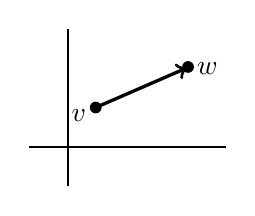
\begin{tikzpicture}[scale=0.5]
            \draw[thick,-] (-1,0) -- (4,0);
            \draw[thick,-] (0,-1) -- (0,3);
            \draw[very thick,->] (0.7,1) -- (3,2) node[right]{$w$};
            \node[inner sep=1.5pt,fill,circle] at (0.7,1) {};
            \node[inner sep=1.5pt,fill,circle] at (3*1.015,2*1.015) {};
            \node[left] at (0.7,0.8){$v$};
            \end{tikzpicture}
            \caption{Un vector afín.}
            \label{fig-vector-afin}
        \end{figure}
        Definimos un \textit{vector afín}\index{vector afín} como un par ordenado de puntos  $v$ y $w$, que escribimos $\overrightarrow{vw}$ y lo visualizamos como una flecha entre $v$ y $w$. Llamamos a $v$ el \textit{punto inicial}\index{vector afín!punto inicial} y $w$ el \textit{punto final}\index{vector afín!punto final} del vector afín (fig. \ref{fig-vector-afin}).
        
        
        
        Sean $\overrightarrow{vw}$ y $\overrightarrow{pq}$ dos vectores afines. Diremos que son \textit{equivalentes}\index{vector afín!equivalencia} si $w-v= q-p$. 
        \begin{figure}[h]
        	\centering
            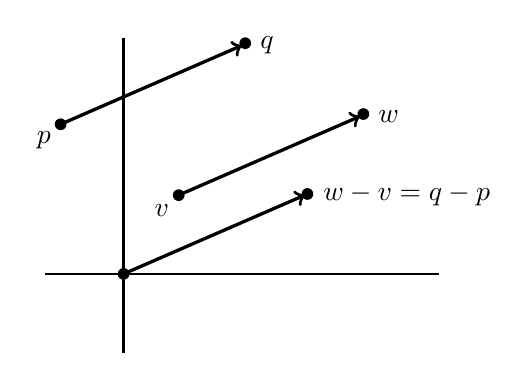
\begin{tikzpicture}
            \draw[thick,-] (-1,0) -- (4,0);
            \draw[thick,-] (0,-1) -- (0,3);
            \draw[very thick,->] (0.7,1) -- (3,2) node[right]{\;$w$};
            \node[inner sep=1.5pt,fill,circle] at (0.7,1) {};
            \node[inner sep=1.5pt,fill,circle] at (3*1.015,2*1.015) {};
            \node[left] at (0.7,0.8){$v$};
            \draw[very thick,->] (0.7-1.5,1+0.9) -- (3-1.5,2+0.9) node[right]{\;$q$};
            \node[inner sep=1.5pt,fill,circle] at (0.7-1.5,1+0.9) {};
            \node[inner sep=1.5pt,fill,circle] at (3*1.015-1.5,2*1.015+0.9) {};
            \node[left] at (0.7-1.5,0.8+0.9){$p$};
            \draw[very thick,->] (0,0) -- (3-0.7,2-1) node[right]{\;$w-v=q-p$};
            \node[inner sep=1.5pt,fill,circle] at (0,0) {};
            \node[inner sep=1.5pt,fill,circle] at (2.3*1.015,1*1.015) {};
            \end{tikzpicture}
            \caption{Dos vectores equivalentes.}
            \label{fig-vectores-equivalerntes}
        \end{figure}
        
        Cada vector afín $\overrightarrow{vw}$ es equivalente a uno cuyo punto de inicial es el origen, pues $\overrightarrow{vw}$ es equivalente a $\overrightarrow{0(w-v)}$ (ver fig. \ref{fig-vectores-equivalerntes}).
        
        Claramente este es el único vector cuyo punto inicial es el origen y que es equivalente a $\overrightarrow{vw}$. Si visualizamos la ley del paralelogramo en el plano, entonces está claro que la equivalencia de dos vectores afines se puede interpretar geométricamente diciendo que las longitudes de los segmentos de línea determinadas por el par de puntos son iguales, y que las ``direcciones'' de los dos vectores son las mismos. 
        
        A una $n$-tupla  la podemos interpretar como un  vector cuyo punto inicial es el origen. En vista de esto, llamaremos, como lo venimos haciendo,  a una $n$-tupla punto o vector, dependiendo de la interpretación que tenemos en mente.
        
        Se dice que dos vectores afines $\overrightarrow{vw}$ y $\overrightarrow{pq}$ son \textit{paralelos} si hay un 	número $\lambda\ne 0$  tal que $w-v= \lambda(q-p)$. Se dice que tienen la \textit{misma dirección} si hay un número $\lambda >0$ tal que $w-v= \lambda(q-p)$, y que tienen \textit{direcciones opuestas} si hay un número $\lambda <0$ tal que $w-v= \lambda(q-p)$.
        
        En los siguientes dibujos, ilustramos vectores afines paralelos. En el primer dibujo  con la misma dirección,  en el segundo, con direcciones opuestas.
        
        
        \begin{center}
            \begin{tabular}{lcl}
                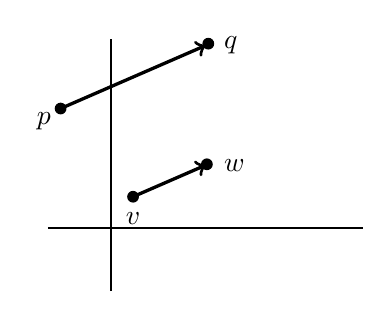
\begin{tikzpicture}[scale=0.8]
                \draw[thick,-] (-1,0) -- (4,0);
                \draw[thick,-] (0,-1) -- (0,3);
                \draw[very thick,->] (0.5*0.7,0.5*1) -- (0.5*3,0.5*2) node[right]{\;$w$};
                \node[inner sep=1.5pt,fill,circle] at (0.5*0.7,0.5*1) {};
                \node[inner sep=1.5pt,fill,circle] at (0.5*3*1.015,0.5*2*1.015) {};
                \node[below] at (0.5*0.7,0.5*0.8){$v$};
                \draw[very thick,->] (0.7-1.5,1+0.9) -- (3-1.5,2+0.9) node[right]{\;$q$};
                \node[inner sep=1.5pt,fill,circle] at (0.7-1.5,1+0.9) {};
                \node[inner sep=1.5pt,fill,circle] at (3*1.015-1.5,2*1.015+0.9) {};
                \node[left] at (0.7-1.5,0.8+0.9){$p$};

                \end{tikzpicture} & 
                \qquad & 
                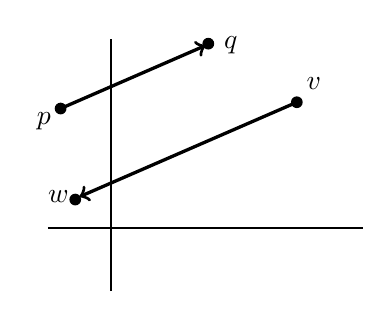
\begin{tikzpicture}[scale=0.8]
                \draw[thick,-] (-1,0) -- (4,0);
                \draw[thick,-] (0,-1) -- (0,3);
                \draw[very thick,->] (-1.5*0.7+4,-1.5*1+3.5) -- (-1.5*3+4,-1.5*2+3.5) node[left]{\;$w$};
                \node[inner sep=1.5pt,fill,circle] at (-1.5*0.7+4,-1.5*1+3.5) {};
                \node[inner sep=1.5pt,fill,circle] at (-1.5*3*1.015+4,-1.5*2*1.015+3.5) {};
                \node[right] at (-1.5*0.7+4,-1.5*0.8+3.5){$v$};
                \draw[very thick,->] (0.7-1.5,1+0.9) -- (3-1.5,2+0.9) node[right]{\;$q$};
                \node[inner sep=1.5pt,fill,circle] at (0.7-1.5,1+0.9) {};
                \node[inner sep=1.5pt,fill,circle] at (3*1.015-1.5,2*1.015+0.9) {};
                \node[left] at (0.7-1.5,0.8+0.9){$p$};
                
                \end{tikzpicture}
            \end{tabular}
        \end{center}

        
    \subsection*{$\S$ Ejercicios}
    
    \begin{enumex}

        \item En  cada uno de los siguientes casos determinar si los
        vectores  $\overrightarrow{vw}$ y $\overrightarrow{xy}$ son
        equivalentes y/o paralelos.
        \begin{enumex}
        \item   $v=(1,-1)$,  $w=(4,3)$, $x=(-1,5)$, $y=(5,2)$. 
        \item   $v=(1,-1,5)$,  $w=(-2,3,-4)$,  $x=(3,1,1)$,  $y=(-3,9,-17)$.
        \end{enumex}
    \end{enumex}

    \end{section}


    \end{section}

    \begin{section}{Rectas en $\R^2$}\label{seccion-rectas-en-r2}
    Conocemos de la secundaria y de cursos anteriores el concepto de recta, por ejemplo en el  sitio online EcuRed dice: 
    
    \textit{``Una recta puede ser expresada mediante una ecuación del tipo $y = m x + b$, donde $x$, $y$ son variables en un plano. En dicha expresión $m$ es denominada pendiente de la recta y está relacionada con la inclinación que toma la recta respecto a un par de ejes que definen el Plano. Mientras que $b$ es el término independiente y es el valor del punto en el cual la recta corta al eje vertical en el plano.''}
    
    Dicho en otros términos una recta,  según esta definición, es el conjunto de puntos $(x,y) \in \R^2$ que satisfacen la ecuación $y = m x + b$ y puede verse como el gráfico de la función $f(x) = m x + b$. Si, por ejemplo, $m=\frac12$ y $b=1$, podemos dibujar la recta en el plano cerca del origen, como en fig.\ref{fig-recta-funcion}.
    \begin{figure}[h]
    	\centering
        \begin{tikzpicture}
        \draw[thick,->] (-4.0,0) -- (4.0,0) node[right] {$x$}; % eje x
        \draw[thick,->] (0,-2) -- (0,3) node[above] {$y$}; % eje y
        \foreach \x in {-2,...,-1} \draw (\x,3pt) -- (\x,-3pt) node[anchor=north] {\x};
        \foreach \x in {1,...,3} \draw (\x,3pt) -- (\x,-3pt) node[anchor=north] {\x};
        \foreach \y in {-1,...,-1} \draw (3pt,\y) -- (-3pt,\y) node[anchor=east] {\y}; 
        \foreach \y in {1,...,2} \draw (3pt,\y) -- (-3pt,\y) node[anchor=east] {\y}; 
        \draw[scale=1,domain=-3:3,smooth,variable=\x,blue] plot ({\x},{0.5*\x +1});
        \end{tikzpicture}
        \caption{La recta $y = \frac12x +1$.}
        \label{fig-recta-funcion}
    \end{figure} 
    
    Sin embargo, con la definición anterior no es posible considerar las rectas verticales. Las rectas verticales están dadas por una ecuación del tipo $x= b$,  es decir son todos los puntos $(x,y)$  tal que $x=b$ e $y$ puede tomar cualquier valor. Por ejemplo, la recta $x=2.5$ se  grafica  como en la fig. \ref{fig-recta-vertical}.
    \begin{figure}[h]
    	\centering
        \begin{tikzpicture}
        \draw[thick,->] (-4.0,0) -- (4.0,0) node[right] {$x$}; % eje x
        \draw[thick,->] (0,-2) -- (0,3) node[above] {$y$}; % eje y
        \foreach \x in {-2,...,-1} \draw (\x,3pt) -- (\x,-3pt) node[anchor=north] {\x};
        \foreach \x in {1,...,3} \draw (\x,3pt) -- (\x,-3pt) node[anchor=north] {\x};
        \foreach \y in {-1,...,-1} \draw (3pt,\y) -- (-3pt,\y) node[anchor=east] {\y}; 
        \foreach \y in {1,...,2} \draw (3pt,\y) -- (-3pt,\y) node[anchor=east] {\y}; 
        \draw[scale=1,domain=-2:3,smooth,variable=\x,blue] plot ({2.5},{\x});
        \end{tikzpicture}
        \caption{La recta $x=2.5$.}
        \label{fig-recta-vertical}
    \end{figure} 
    
    No es difícil dar una definición que englobe todas las rectas posibles del plano:
    
    \begin{definicion}[Definición general de la recta] Sean  $a,b,c \in \R$ y tal que $a,b$ no son simultáneamente $0$. La \textit{recta con ecuación implícita}\index{recta en $\R^2$} \index{recta en $\R^2$!ecuación implícita}
    \begin{equation}\label{eq-implicita-de-la-recta}
        ax +by =c,
    \end{equation}
    es el conjunto de puntos $(x,y)$ en $\R^2$ que satisfacen la ecuación \eqref{eq-implicita-de-la-recta}.  Es decir, si denotamos $L$  a la recta,
    \begin{equation*}
        L = \{ (x,y)\in \R^2: ax +by =c\}.
    \end{equation*}
    \end{definicion}


    Observar  que si $b\ne0$, entonces la recta es \, $y= -\displaystyle\frac{a}{b}x + \displaystyle\frac{c}{b}$ \, y que si $b=0$,  entonces $a\ne 0$ y la recta es \, $x =\displaystyle\frac{c}{a}$.
    
    \begin{observacion*}
        Si  consideramos  el vector $(a,b)$ en $\R^2$, $c \in \R$ y $L$ la recta definida por los puntos $(x,y)$ tal que $ax +by =c$,  entonces $L$ es la recta formada por el conjunto de puntos $(x,y)$ en $\R^2$ que satisfacen 
        \begin{equation*}
            \langle (x,y), (a,b) \rangle = c.
        \end{equation*}
    Ahora bien, consideremos $(x_0,y_0)$ un punto de la recta, entonces,  obviamente tenemos que $\langle (x_0,y_0), (a,b) \rangle = c$, por lo tanto la recta se puede describir como los puntos $(x,y)$ que satisfacen la ecuación 
    \begin{equation*}
    \langle (x,y), (a,b) \rangle = \langle (x_0,y_0), (a,b) \rangle.
    \end{equation*}	
    Por la propiedad \ref{prop-P2} del producto escalar, llegamos a la conclusión que 
    \begin{equation*}
    L = \{(x,y) \in \R^2: \langle (x,y)-(x_0,y_0)\,,\, (a,b) \rangle = 0 \}.
    \end{equation*}
    Sea $v_0 =(x_0,y_0)$ y $v =(x,y)$,   representemos gráficamente la situación: 
    \begin{figure}[h]
    	\centering
        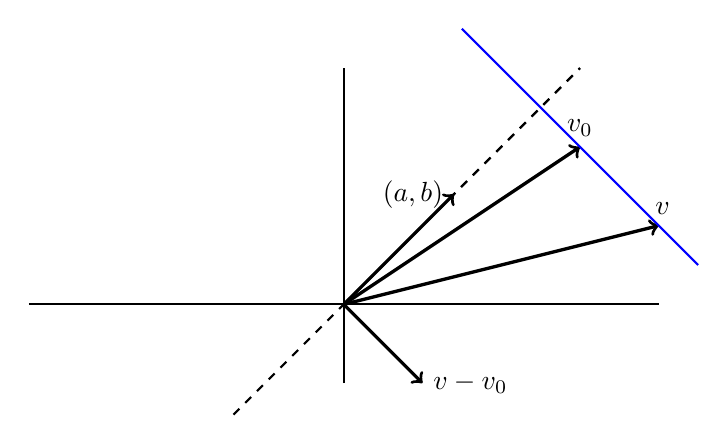
\begin{tikzpicture}
        \def\vx{3}
        \def\vy{2}
        \def\wx{4}
        \def\wy{1}	
        \def\tv{3.0}
        \def\tw{1.4}
        \def\taa{1.5}
        \def\tab{-1.5}
        \def\rr{\tv*\vy-\tv*\wy}	
        \def\ss{\tv*\wx-\tv*\vx}		
        \def\rrm{-\tw*\vy+\tw*\wy}	
        \def\ssm{-\tw*\wx+\tw*\vx}		
        \draw[thick,-] (-4,0) -- (4,0);
        \draw[thick,-] (0,-1) -- (0,3);
        %\node[inner sep=1.5pt,fill,circle] at (\vx,\vy) {};
        \draw[very thick,->] (0,0) -- (\vx,\vy) node[above]{$v_0$};
        \draw[very thick,->] (0,0) -- (\wx,\wy) node[above]{\;$v$};
        \draw[very thick,->] (0,0) -- (\wx-\vx,\wy-\vy) node[right]{$v-v_0$};
        \draw[thick,blue,-] (\vx- \tab*\vx + \tab*\wx ,\vy - \tab*\vy + \tab*\wy) --  (\vx- \taa*\vx + \taa*\wx ,\vy - \taa*\vy + \taa*\wy);
        \draw[very thick,->] (0,0) -- (\tw*\vy-\tw*\wy,\tw*\wx-\tw*\vx) node[left]{$(a,b)$};
        \draw[dashed, thick,-] (0,0) -- (\rr,\ss);
        \draw[dashed, thick,-] (0,0) -- (\rr,\ss);
        \draw[dashed, thick,-] (\rrm,\ssm) -- (0,0);
        %\draw[dashed,thick] (0,0) (\tw*\wx,\tw*\wy) -- (\vx+\tw*\wx,\vy+\tw*\wy+0.1);
        %\node[inner sep=1.5pt,fill,circle,blue] at (\vx+\tw*\wx+0.04*\wx,\vy+\tw*\wy+0.04*\wy)  {};
        %\node[right] at (\vx+\tw*\wx,\vy+\tw*\wy+0.1){$v+tw$};
        \end{tikzpicture}
        \caption{Una recta en el plano.}
        \label{fig-recta-parametrica}
    \end{figure} 


    La recta $L$ es, entonces, la recta perpendicular a $(a,b)$ y que pasa por $v_0$. 
    
    \end{observacion*}

    El  razonamiento también es posible hacerlo en el otro sentido: 

    \begin{resultado}\label{res-recta-perp}
        {La ecuación implícita de la recta $L$ perpendicular a $(a,b)$ y que pasa por $(x_0,y_0)$ es
            \begin{equation*}
            ax +by = \langle (x_0,y_0), (a,b) \rangle.
            \end{equation*}}
    \end{resultado}

\begin{ejemplo*}
    Encontrar la ecuación implícita de la recta que pasa por $(2,-1)$ y  es perpendicular a $(-2,3)$.
\end{ejemplo*}
\begin{proof}[Solución]
Por lo visto anteriormente la recta esta formada por los puntos  $(x,y)$ tales que
    \begin{equation*}
            -2x+3y = c
    \end{equation*}
     y debemos determinar el valor de $c$. Como $(2,-1)$ pertenece a la recta
     \begin{equation*}
     c = -2\cdot 2+3\cdot (-1) = -7.
     \end{equation*}
     Luego, la ecuación implícita de la recta es
     \begin{equation*}
     -2x+3y = -7.
     \end{equation*}
\end{proof}


    Una definición equivalente de recta es la siguiente:
    
        \begin{definicion}
            Sean $v, w \in \R^2$ tal que  $w \not=0$. Sea 
            \begin{equation*}
            L = \{v + tw: t \in \R\}. 
            \end{equation*}
            Diremos entonces que  \textit{$L$ es la recta que pasa por $v$ paralela a $w$.} 
        \end{definicion}
        
    Observemos que la recta $L$ está dada por todos los puntos que se obtienen de la función
    \begin{equation}\label{eq-ecuacion-parametrica-recta}
    X(t) =v +tw, \quad \text{para $t \in \R$.} 
    \end{equation} 
    En  el espacio $\R^2$, diremos que \eqref{eq-ecuacion-parametrica-recta} es la \textit{ecuación paramétrica} o la \textit{representación paramétrica}\index{recta en $\R^2$!ecuación paramétrica} de la recta $L$ que pasa por el punto $v$ y es paralela a $w \ne 0$.
        



        
        Podemos representar una recta dada en forma paramétrica como en la figura \ref{fig-recta-parametrica}.
        \begin{figure}[h]
        	\centering
            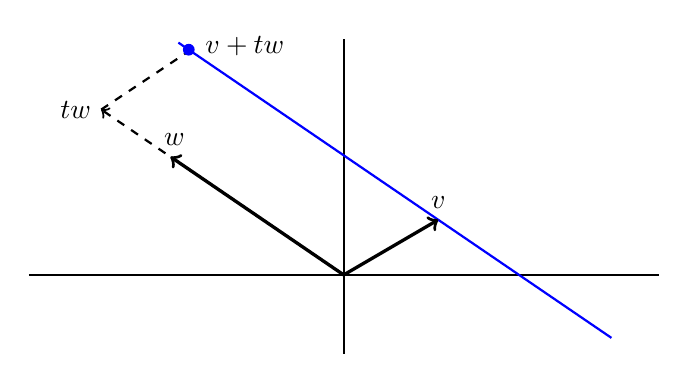
\begin{tikzpicture}
            \def\vx{1.2}
            \def\vy{0.7}
            \def\wx{-2.2}
            \def\wy{1.5}	
            \def\tw{1.4}					
            \draw[thick,-] (-4,0) -- (4,0);
            \draw[thick,-] (0,-1) -- (0,3);
            \draw[thick,blue,-] (\vx+1.5*\wx,\vy+1.5*\wy) -- (\vx-1*\wx,\vy-1*\wy);
            %\node[inner sep=1.5pt,fill,circle] at (\vx,\vy) {};
            \draw[very thick,->] (0,0) -- (\vx,\vy) node[above]{$v$};
            \draw[very thick,->] (0,0) -- (\wx,\wy) node[above]{\;$w$};
            \draw[dashed, thick,->] (0,0) -- (\tw*\wx,\tw*\wy) node[left]{$tw$};
            \draw[dashed,thick] (0,0) (\tw*\wx,\tw*\wy) -- (\vx+\tw*\wx,\vy+\tw*\wy+0.1);
            \node[inner sep=1.5pt,fill,circle,blue] at (\vx+\tw*\wx+0.04*\wx,\vy+\tw*\wy+0.04*\wy)  {};
            \node[right] at (\vx+\tw*\wx,\vy+\tw*\wy+0.1){$v+tw$};
            \end{tikzpicture}
            \caption{Una recta en el plano.}
            \label{fig-recta-parametrica}
        \end{figure} 
        Cuando damos tal representación paramétrica, podemos pensar en un móvil que comienza en el punto $v$ en el tiempo $t = 0$, y moviéndose en la dirección de $w$. En el momento $t$, el móvil está en la posición $v+tw$. Por lo tanto, podemos interpretar físicamente la representación paramétrica como una descripción del movimiento, en que $w$ se interpreta como la velocidad del móvil. En un momento dado $t$, el móvil está en el punto $X(t) =v +tw$ que es  llamada la \textit{posición} del móvil en el tiempo $t$.
        
        Esta representación paramétrica también es útil para describir el conjunto de los puntos que se encuentran en el segmento de línea entre dos puntos dados. Sean $v$, $u$ dos puntos, entonces el segmento entre $v$ y $u$ consiste en todos los puntos
        \begin{equation}\label{eq-segmento-parametrico}
            S(t) = v + t(u-v)\quad  \text{con}\quad 0 \le t \le 1.
        \end{equation}
        Observar que en tiempo 0, $S(0) = v$ y  en tiempo 1, $S(1)= v + (u-v)= u$. Como $t$ ``va'' de 0 a 1,  el móvil va de $v$ a $u$,  en linea recta. %En  el lenguaje de vectores afines, \eqref{eq-segmento-parametrico} es \textit{la ecuación paramétrica del vector $\overrightarrow{vu}$}.
        
        Extendiendo a ambos lados el segmento, podemos describir la recta que pasa por $v$ y $u$ por la ecuación paramétrica (fig. \ref{fig-recta-entre-puntos})
        \begin{equation*}
        S(t) = v + t(u-v)\quad  \text{con}\quad t \in \R.
        \end{equation*}
        \begin{figure}[h]
        	\centering
            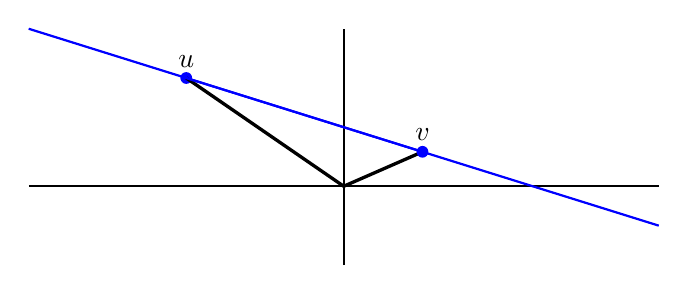
\begin{tikzpicture}
            \draw[thick,-] (-4,0) -- (4,0);
            \draw[thick,-] (0,-1) -- (0,2);
            \draw[blue,-] (-4,2) -- (4,-0.5);
            \node[inner sep=1.5pt,fill,circle,blue] at (-4 + 8/4,2 -2.5/4) {};
            \draw[very thick,-] (0,0) -- (-4 + 8/4,2 -2.5/4) node[above]{$u$};
            \draw[very thick,-] (0,0) -- (-4 + 2.5*8/4,2 -2.5*2.5/4) node[above]{$v$};
            \node[inner sep=1.5pt,fill,circle,blue] at (-4 + 2.5*8/4,2 -2.5*2.5/4)  {};
            \draw[thick,blue,-] (-4 + 8/4,2 -2.5/4) -- (-4 + 2.5*8/4,2 -2.5*2.5/4);
            \draw[thick,blue,-] (-4,2) -- (4,-0.5);
            \end{tikzpicture}
            \caption{La recta que pasa por $v$ y $u$.}
            \label{fig-recta-entre-puntos}
        \end{figure} 
        
        \begin{ejemplo*}
            Encontrar una representación paramétrica para la recta que contiene los puntos $(1, - 3, 1)$ y $(- 2,4,5)$.
        \end{ejemplo*}	
        \begin{proof}[Solución] Llamemos $v = (1, - 3, 1)$ y $u =(- 2,4,5)$. Entonces $$u-v = (- 2,4,5) - (1,-3,1) = (-3,7,4)$$ y la representación paramétrica de la recta que pasa por $u$ y $v$  es 
        \begin{equation*}
            X (t) = v + t(u-v) = (1, -3,1) + t (-3, 7, 4),\quad t\in \R.
        \end{equation*}
        \end{proof}
    
        Ahora discutiremos la relación entre una representación paramétrica y la ecuación implícita de una recta en el plano.
        
        Supongamos que trabajamos en el plano y tenemos $v, w \in \R^2$ con $w \not= 0$ y la recta descrita en forma paramétrica:
        \begin{equation*}
        X(t) =v +tw.
        \end{equation*}
        Sea $v = (x_1,y_1)$, $w = (x_2,y_2)$,  entonces, todo punto de la recta es de la forma
        \begin{equation*}
        (x,y) =(x_1,y_1) +t(x_2,y_2) = (x_1+tx_2,y_1+ty_2),
        \end{equation*}
        es decir, los puntos de la recta $X$ son los $(x,y)$ tal que
        \begin{equation*}
            x = x_1+tx_2, \qquad y = y_1+ty_2, \qquad
        \end{equation*}
        para $t \in \R$. Dado  que $(x_2,y_2) \ne 0$, podemos despejar $t$  de alguna de las ecuaciones y usando la otra ecuación eliminamos $t$ y obtenemos una ecuación implícita. Veremos esto en un ejemplo.
        
        \begin{ejemplo*}
            Sean $v = (2, 1)$ y $w = (- 1, 5)$ y sea $X$ la recta que pasa por $v$  en la dirección $w$. Encontrar la ecuación  implícita de $L$.
    \end{ejemplo*}
\begin{proof}[Solución]	
            La representación paramétrica de la recta que pasa por  $v$ en la dirección de $w$ es 
            \begin{equation*}
                X(t)= (2,1)+ t(-1,5) = (2-t,1+5t).
            \end{equation*}
             Es decir, si  miramos cada coordenada, 
            \begin{equation}\label{eq-par-des-ej}
            x = 2 - t, \qquad\quad y = 1 + 5t.
            \end{equation}
            Despejando $t$ de la primera ecuación obtenemos $t = 2-x$. Reemplazando este valor de $t$  en la segunda ecuación obtenemos $y = 1 + 5t=1 + 5(2-x)t= y = 11- 5x$, luego
            \begin{equation}\label{eq-impl-rec-ej}
                5x + y = 11,
            \end{equation}
            que es la ecuación implícita de la recta.
            
            \end{proof}	
            
            Esta eliminación de $t$ muestra que cada par $(x, y)$ que satisface la representación paramétrica \eqref{eq-par-des-ej} para algún valor de $t$ también satisface la ecuación \eqref{eq-impl-rec-ej}.
            
            Recíprocamente, de la ecuación implícita podemos obtener la representación paramétrica. 
            
            \begin{ejemplo*} Encontrar la representación paramétrica de la recta definida por 
                \begin{equation*}
                5x + y = 11. 
                \end{equation*}
            \end{ejemplo*}
            \begin{proof}[Solución]
                 Supongamos que tenemos un par de números $(x, y)$ que satisfacen la ecuación  implícita, $5x + y = 11$, luego $y = (-5)x + 11$, remplazando $x$ por $t$ (sólo por notación) obtenemos que 
                 \begin{equation*}
                     Y(t) = (t, -5t+11)
                 \end{equation*}
                es la representación paramétrica de la recta.
        \end{proof}	 
    

     
     De los ejemplos anteriores se deduce que la recta 
     \begin{equation*}
         X(t)=  (2-t,1+5t)
     \end{equation*}
     es la misma que la recta 
     \begin{equation*}
         Y(t) = (t, -5t+11).
     \end{equation*}     
     Observar que, pese a que hablamos de ``la representación paramétrica de la recta'', una recta tiene muchas formas de ser representada paramétricamente. 
    
        Los procedimientos  de los ejemplos anteriores se pueden generalizar a cualquier recta y de esa forma se puede demostrar que la definición paramétrica y la definición implícita de la recta son equivalentes. 
        
        Finalmente, podemos obtener la representación paramétrica de la recta a partir de un vector ortogonal a ella y otro vector perteneciente a ella. 
                
        \begin{proposicion}
            Sean $(a,b),(x_0,y_0)\in\R^2$ con $(a,b)\neq0$.  La recta perpendicular a $(a,b)$ que pasa por $(x_0,y_0)$ es
            \begin{align*}
            L=\left\{(x_0,y_0)+t(b,-a)\mid t\in\R\right\} 
            \end{align*}
        \end{proposicion}
    \begin{proof}
    El vector $(b,-a)$  es perpendicular a a $(a,b)$  y por lo tanto tiene la dirección de la recta. Luego  la ecuación paramétrica de la recta es $v_0+t(b,-a)$ para algún $v_0$  en la recta. Como $(x_0,y_0)$ pertenece a la recta, obtenemos el resultado que queríamos probar.
    \end{proof}
        

\begin{ejemplo*}
    Encontrar una representación paramétrica para la recta que contiene los puntos $(2,2)$ y y es perpendicular a $(2,1)$.
\end{ejemplo*}	
\begin{proof}[Solución]

    El vector ortogonal a $(2,1)$  es $(1,-2)$. Luego:
    
    \begin{align*}
    L&=\left\{(2,2)+t(1,-2)\mid t\in\R\right\} \\
    &= \left\{(2 +t,2-2t)\mid t\in\R\right\}
    \end{align*}

\end{proof}


        
        
        Debemos observar que en $\R^3$ no alcanza una sola ecuación lineal del tipo $ax+by+cz=d$ para definir una recta. Veremos en la sección siguiente que una ecuación lineal define un plano en $\R^3$. Genéricamente hablando, con las soluciones de una ecuación en $\R^n$ se obtiene un objeto ``con una dimensión menos''. Todo esto quedará claro al final de la materia cuando estudiemos subespacios vectoriales de un espacio vectorial. 
	


    \subsection*{$\S$ Ejercicios}
    
    \begin{enumex}

        
        \item Sea $R_1$ la recta que pasa por $p_1=(2,0)$ y es ortogonal a $(1,3)$.
        \begin{enumex}
         \item Dar la descripción paramétrica e implícita de $R_1$.
         \item Graficar en el plano a $R_1$.
         \item Dar un punto $p$ por el que pase $R_1$ distinto a $p_1$.
         \item Verificar si $p+p_i$ y $-p$ pertenece a $R_1$
        \end{enumex}
        
        \vskip .2cm
        
        \item Repetir el ejercicio anterior con las siguientes rectas.
        \begin{enumex}
            \item
            $R_2$: recta que pasa por $p_2=(0,0)$ y es ortogonal a $(1,3)$.
            \item
            $R_3$: recta que pasa por $p_3=(1,0)$ y es paralela a $R_1$.
        % 	\item
        % 	$R_4$: recta que pasa por los puntos $(-1,5,4)$ y $(0,3,-2)$.
        \end{enumex}
        
        \vskip .2cm
        
        \item Calcular, numérica y gráficamente, las intersecciones $R_1\cap R_2$ y $R_1\cap R_3$. 
        \vskip .2cm
        
        \item Sea $L=\{(x,y)\in\R^2 : ax+by=c\}$ una recta en $\R^2$. Sean $p$ y $q$ dos puntos por los que pasa $L$.
        \begin{enumex}
         \item ¿Para qué valores de $c$ puede asegurar que $(0,0)\in L$?
         \item ¿Para qué valores de $c$ puede asegurar que $\lambda q\in L$?, donde $\lambda\in\R$.
         \item ¿Para qué valores de $c$ puede asegurar que $p+q\in L$?
        \end{enumex}
        
        
        \vskip .2cm
        
        \item Sea $L$ una recta en $\R^2$. Probar que $L$ pasa por $(0,0)$ si y solo si pasa por $p+\lambda q$ para todo par de puntos distintos $p$ y $q$ de $L$ y para todo $\lambda\in\R$.
\end{enumex}

    
    \end{section}



    \begin{section}{Planos en $\R^3$}\label{seccion-planos-en-r3} 
        En  la sección anterior vimos (aunque no lo demostramos) que existe una equivalencia entre la definición implícita y la definición paramétrica de la recta. En esta sección definiremos un plano en $\R^3$ utilizando la forma implícita, que es la forma más usual y además es geométricamente intuitiva. Luego veremos la definición del plano en su versión paramétrica . 
        
        Comenzaremos, debido a que es más simple, con planos que  pasan por el origen,  como el de la fig. \ref{fig-plano-por-origen}.
        \begin{figure}[h]
        	\centering
            \begin{tikzpicture}[plane/.style={trapezium,draw,fill=black!20,trapezium left angle=60,trapezium right angle=120,minimum height=1.5cm},scale=0.7]
            \node (p)[plane,rotate=-30] at (0,0){.};
            \draw[rotate=-30] (p.center) edge ++(0,2cm) edge[densely dashed] (p.south) (p.south) edge ++(0,-1cm);
            \draw[->] (0,0,0) -- (2*0.5,2*0.866,0) node[right]{$u$};
            \draw[thick,->] (0,0,0) -- (3,0,0) node[right]{$y$};
            \draw[thick,->] (0,0,0) -- (0,2.5,0) node[above]{$z$};
            \draw[thick,->] (0,0,0) -- (0,0,3) node[anchor=north east]{$x$};
            \node [right] at (1.2,-0.1,1.5) {$P$};
            \end{tikzpicture}
            \caption{El plano $P$ y $u$, un vector  perpendicular al plano.}
            \label{fig-plano-por-origen}
        \end{figure} 
    
        En  este caso,  es claro que el plano está determinado por un vector perpendicular al mismo, es decir si $P$  es un plano que pasa por el origen y $u$ es un punto de $\R^3$, no nulo, tal que $u \perp P$,  entonces
        \begin{equation*}
            P = \{ v \in \R^3: \la v,u \ra=0 \}. 
        \end{equation*}
        Sea ahora un  plano $P$ que no pasa por el origen.  Tomo $v_0 \in P$ y entonces observamos que
        \begin{equation}\label{eq-p0-plano-1}
            P_0 = \{v-v_0: v \in P \}
        \end{equation} 
        es un plano que pasa por el origen (pues $v_0-v_0 \in P_0$). Luego,  si $u$ perpendicular a $P_0$ tenemos que
        \begin{equation}\label{eq-p0-plano-2}
        P_0 = \{w: \la w,u \ra=0\}.
        \end{equation}
        De las ecuaciones \eqref{eq-p0-plano-1} y  \eqref{eq-p0-plano-2} deducimos que 
        \begin{equation*}
            v \in P \Leftrightarrow v-v_0 \in P_0 \Leftrightarrow \la v-v_0,u \ra=0,
        \end{equation*}
         es decir
        \begin{equation*}
            P = \{ v \in \R^3: \la v-v_0,u \ra=0 \}. 
        \end{equation*}  
        Observemos que  $\la v-v_0,u \ra=0$ sii $\la v,u \ra-\la v_0,u \ra=0$ sii $\la v,u \ra=\la v_0,u \ra$. Es decir, si $d = \la v_0,u \ra$, tenemos
        \begin{equation*}
        P = \{ v \in \R^3: \la v,u \ra=d \}. 
        \end{equation*} 
        
        Esta interpretación geométrica del plano se puede formalizar en la siguiente definición.
        
        
        \begin{definicion}\label{def-eq-implicita-plano} Sean $a,b, c,d \in \R$ tal que $(a,b,c) \ne (0,0,0)$ y sea 
        \begin{equation*}
            P = \{(x,y,z): ax +by +cz =d\}.
        \end{equation*}
        Entonces diremos que $P$  es  un \textit{plano con ecuación implícita}\index{plano en $\R^3$!ecuación implícita}  $ax +by +cz =d$ y  que $(a,b,c)$ es un \textit{vector normal al plano $P$.} A esta forma de describir el plano también suele llamársela la \textit{ecuación normal del plano.}\index{plano en $\R^3$!ecuación normal}
        \end{definicion} 
        
        Observar que la ecuación $ ax +by +cz =d$ no es más que la ecuación $\la(x,y,z),(a,b,c) \ra=d$. 	
        
        \begin{ejemplo*}
            El plano determinado por la ecuación
            \begin{equation*}
                2x - y 	+ 3z = 	5
            \end{equation*}
            es perpendicular al vector $(2, - 1, 3)$. Si queremos encontrar un punto en ese plano, por supuesto que tenemos muchas opciones. Podemos dar un valor arbitrario a $x$ e $y$, y luego despejamos $z$. Para obtener un punto concreto, sea $x = 1$, $y = 1$. Luego resolvemos para $z$, a saber
            \begin{equation*}
                3z 	= 5 - 2 + 1 = 4,
            \end{equation*}
            luego $z = \displaystyle\frac43$ y entonces
            \begin{equation*}
                (1,1,\frac43)
            \end{equation*}
            es un punto en el plano.
        \end{ejemplo*}
        
        Se dice que dos planos son \textit{paralelos} (en el 3-espacio) si sus vectores normales son paralelos,  es decir son proporcionales. Se dice que son \textit{perpendiculares} si sus vectores normales son perpendiculares. El \textit{ángulo entre dos planos} se define como el ángulo entre sus vectores normales.
        
        
        
        Como $(a,b,c) \ne (0,0,0)$,  entonces una de las tres componentes del vector normal al plano no es cero. Supongamos que $a\ne 0$,  luego es fácil despejar $x$ en función de las constantes $a$, $b$, $c$ y $d$; y las variables $y$ y $z$, por lo tanto cada coordenada del plano depende paramétricamente de $y$ y $z$ y así obtenemos una ecuación paramétrica de $P$ (que depende de 2 parámetros). Se puede hacer de forma análoga cuando $b\ne 0$ o $c \ne 0$. 
        
        \begin{ejemplo*}
            Dado el plano $P = \{(x,y,z): x -2y +z =1\}$,  hallaremos una ecuación paramétrica de $P$. Como  $x -2y +z =1$ sii  $x = 2y-z +1$, tenemos que
            \begin{equation*}
                P = \{(2y-z +1,y,z): y,z \in \R\},
            \end{equation*}
            o,  escrito de una forma más estándar,
            \begin{equation*}
            P = \{(2s-t +1,s,t): s,t \in \R\}. 
            \end{equation*}
            Observemos que 
            \begin{align*}
                (2s-t +1,s,t) &= (1,0,0) + (2s-t,s,t)\\
                &= (1,0,0) + (2s,s,0) + (-t,0,t)\\
                & = (1,0,0) + s(2,1,0) + t(-1,0,1),
            \end{align*}
            por lo tanto, podemos también escribir
            \begin{equation*}
            P = \{(1,0,0) + s(2,1,0) + t(-1,0,1): s,t \in \R\}. 
            \end{equation*}
            Cualquiera de las formas paramétricas de describir $P$  es correcta, pero la última es la que se utiliza para definir formalmente el plano en forma paramétrica. 
        \end{ejemplo*}
    
    \begin{definicion}
        Sean $v, w_1,w_2 \in \R^3$ tal que  $w_1$,$w_2$ no  nulos y tal que $w_2$ no sea un múltiplo de $w_1$. Sea 
        \begin{equation*}
        P = \{v + sw_1 + tw_2: s,t \in \R\}. 
        \end{equation*}
        Diremos entonces que  \textit{$P$ es el  plano a través de $v$ paralelo a los vectores $w_1$ y $w_2$.}\index{plano en $\R^3$!ecuación paramétrica} 
    \end{definicion}
    
        Claramente,  en la definición de arriba, el vector $v$ pertenece al plano y el plano 
        \begin{equation*}
        P_0 = \{sw_1 + tw_2: s,t \in \R\}
        \end{equation*}
        es el plano que pasa por el origen y paralelo a $P$. 
 
    
    Ya  hemos visto que de la ecuación implícita del plano podemos pasar a al ecuación paramétrica fácilmente. Es un poco menos directo pasar de la ecuación paramétrica a la ecuación implícita, pero podemos describir un procedimiento general: sea $P = \{v + sw_1 + tw_2: s,t \in \R\}$,  entonces $v \in P$ y $P_0 = \{sw_1 + tw_2: s,t \in \R\}$  es el plano paralelo a $P$  que pasa por el origen. Si encontramos $u \ne 0$ tal que $\la u,w_1 \ra =0$ y $\la u,w_2 \ra =0$, entonces $ \la  sw_1 + tw_2, u \ra =0$ para  $s,t$ arbitrarios y 
    \begin{equation*}
    P_0 = \{(x,y,z): \la (x,y,z),u \ra =0\}. 
    \end{equation*}
    Sea $d = \la v, u \ra$, entonces $\la v + sw_1 + tw_2, u\ra = \la v , u\ra =d$, para $s,t$ arbitrarios. Es decir
    \begin{equation*}
    P = \{(x,y,z): \la (x,y,z),u \ra =d\}. 
    \end{equation*}
      
    \begin{ejemplo*}
        Sea $P$ el plano definido en forma paramétrica por 
        \begin{equation*}
            P = \{ (1,1,0) + s(-1,0,-1) + t(0,1,-2): s,t \in \R\}.
        \end{equation*}
         Encontremos la ecuación implícita de  $P$. 
         
         Sea $u= (a,b,c)$,  entonces 
        \begin{align*}
            \la u,(-1,0,-1) \ra = 0 \quad &\Leftrightarrow \quad -a -c=0, \\
            \la u,(0,1,-2) \ra = 0 \quad &\Leftrightarrow \quad b -2c=0.
        \end{align*} 
        Estas dos ecuaciones se cumplen sii $a = -c$ y $b=2c$, es decir si $u=(-c,2c,c)$. Si, por ejemplo, $c=1$, tenemos $u=(-1,2,1)$, luego el plano paralelo a $P$  que pasa por el origen es
        \begin{equation*}
        P_0 = \{(x,y,z): -x+2y+z =0\}. 
        \end{equation*}
        Como $\la (1,1,0),(-1,2,1) \ra = 1 $, obtenemos
        \begin{align*}
        P &= \{(x,y,z): \la (x,y,z),(-1,2,1) \ra =1\} \\
        &= \{(x,y,z): -x+2y+z =1\}.
        \end{align*}
    \end{ejemplo*}

    \subsection*{$\S$ Ejercicios}
    
    \begin{enumex}

         
    \item Sea $v_0=(2,-1,1)$.
        \begin{enumex}
            \item Describir param{\'e}tricamente el conjunto
            $P_1=\{w\in\mathbb{ R}^3:\langle v_0 , w  \rangle=0\}$.
            \item Describir param{\'e}tricamente el conjunto
            $P_2=\{w\in\mathbb{ R}^3:\langle v_0 , w  \rangle=1\}$.
            \item ¿Qu\'e relaci\'on hay entre $P_1$ y $P_2$?
        \end{enumex}
        
        \vskip .2cm
        
    \item\label{ej-planos} Escribir la ecuación paramétrica  y la ecuación normal de los siguientes planos.
        \begin{enumex}
            \item $\pi_1$: el plano que pasa por $(0,0,0)$, $(1,1,0)$, $(1,-2,0)$.
            \item $\pi_2$: el plano que pasa por $(1,2,-2)$ y es perpendicular a la
            recta que pasa por $(2,1,-1)$, $(3,-2,1)$.
            \item\label{ej-planos-c}  $\pi_3=\{w\in\R^3: w=s(1,2,0)+t(2,0,1)+(1,0,0);\,s,t\in \mathbb R\}$.
        \end{enumex}
        
        \vskip .2cm
        
        
    \item ¿Cuáles de las siguientes rectas cortan al plano $\pi_3$ del  ejercicio \ref{ej-planos} \ref{ej-planos-c}?
        Describir la intersección en cada caso.
        \begin{enumex}
            \item $\{w: w=(3,2,1)+t(1,1,1)\}$,
            \item $\{w: w=(1,-1,1)+t(1,2,-1)\}$,
            \item $\{w: w=(-1,0,-1)+t(1,2,-1)\}$, 
            \item $\{w: w=(1,-2,1)+t(2,-1,1)\}$.
        \end{enumex}
\end{enumex}




   \end{section}

   \begin{section}{Bases ortonormales en $\R^n$ (*)}\label{seccion-bases-ortonormales-rn}


    \begin{definicion} \label{def-bo}\label{def-bon}
        Diremos que $\mathcal B =\{u_1,\ldots,u_n\}\subset \R^n$ es una \textit{base ortogonal} o \textit{BO} de $\R^n$ si $u_i \perp u_j$ cuando $i\ne j$. Diremos $\mathcal B$ que es una \textit{base ortonormal} o \textit{BON} si es una base ortogonal y $||u_i||=1$ para todo $i$.\index{base ortogonal!en $\R^n$}  \index{base ortonormal!en $\R^n$}  
    \end{definicion}

    \begin{ejemplo*} 

        \

        \begin{enumerate}
            \item La base canónica $\mathcal C= \{e_1,\ldots,e_n\}$  es una base ortonormal de $\R^n$. 
            \item Cualesquiera dos vectores ortogonales en $\R^2$ forman una base ortogonal, por ejemplo, $(1,-1), (1,1)$.
            \item $\mathcal B_1 = \{(\cos\theta, \sen\theta,0),  (-\sen\theta, \cos\theta,0 ),  (0,0,1)\}$ es una BON  de $\R^3$
            \begin{proof}
                \begin{align*}
                    \la (\cos\theta, \sen\theta,0), (\cos\theta, \sen\theta,0)\ra &= \cos^2\theta+ \sen^2\theta = 1\\
                    \la (-\sen\theta, \cos\theta,0 ),  (-\sen\theta, \cos\theta,0 )\ra &= \sen^2\theta +\cos^2\theta = 1\\
                    \la (0,0,1),  (0,0,1)\ra &=1.
                \end{align*}
                Es decir todos los vectores tiene norma 1. Ahora bien,
                \begin{align*}
                    \la (\cos\theta, \sen\theta,0),  (-\sen\theta, \cos\theta,0 )\ra &= -\sen\theta\cos\theta+ \sen\theta\cos\theta = 0\\
                    \la (\cos\theta, \sen\theta,0),  (0,0,1 )\ra &=0\\
                    \la  (-\sen\theta, \cos\theta,0 ),  (0,0,1 )\ra &=0.
                \end{align*}
                Es decir,  todos los vectores son ortogonales entre sí. Luego $\mathcal B_1$  es una BON.
                
            \end{proof} 
            \item  $\mathcal B_2 = \{(3/5, 4/5,0 ), (- 4/5, 3/5,0),  (0,0,1 )\}$ es una BON  de $\R^3$. 
            
            Esto se prueba en fórma análoga al ítem anterior: primero se verifica que todos los vectores tengan norma 1  y luego que dos vectores distintos en $\mathcal B_2$ sean ortogonales.
        \end{enumerate}
    \end{ejemplo*}

    \begin{obs*}
        Sea  $\mathcal B =\{v_1,\ldots,v_n\}$ una base ortogonal de $\R^n$,  entonces si $u_i = \displaystyle\frac{v_i}{||v_i||}$ el conjunto $\mathcal B' =\{u_1,\ldots,u_n\}$ es una base ortonormal de $\R^n$. 
    \end{obs*}

   
    
    Recordemos que si $\mathcal C= \{e_1,\ldots,e_n\}$ es la base canónica de $\R^n$ y $v =(x_1,\ldots,x_n)$,  entonces 
    $v = x_1 e_1 + x_2 e_2 + \cdots + x_n e_n$. Como $\la v,e_i\ra = x_i$, podemos reescribir 
    \begin{equation*}
        v = \la v,e_1\ra e_1 +\la v,e_2\ra e_2 +\cdots+\la v,e_n\ra e_n.
    \end{equation*} 
    
    
    El siguiente teorema generaliza la fórmula  anterior a cualquier base ortonormal. La prueba la podremos hacer recién en el capítulo \ref{chap-esp-prod-int}.

    \begin{teorema}\label{th-cl-bon}
        Sea $\mathcal B =\{u_1,\ldots,u_n\}$ una BON de $\R^n$, y $v \in \R^n$, entonces
        \begin{equation*}
            v = \la v,u_1\ra u_1 +\la v,u_2\ra u_2 +\cdots+\la v,u_n\ra u_n. \tag*{\qed}
        \end{equation*} 
    \end{teorema}
    
    La facilidad de escribir cualquier vector como combinación lineal de los vectores de una base ortonormal  es una propiedad de suma importancia con aplicaciones en la física y la matemática. 

    \begin{corolario}\label{cor-gm-rn-1}
        Sea $\mathcal B =\{w_1,\ldots,w_n\}$ una BO de $\R^n$, y $v \in \R^n$, entonces
        \begin{equation*}
            v = \frac{\la v,w_1\ra}{ \la w_1, w_1\ra} w_1 +\frac{\la v,w_2\ra}{\la w_2, w_2\ra} w_2 +\cdots+\frac{\la v,w_n\ra}{\la w_n, w_n\ra} w_n. 
        \end{equation*} 
    \end{corolario}
    \begin{proof}
        Como $\{w_1,\ldots,w_n\}$ es una BO,  entonces 
        $\displaystyle\left\{\frac{w_1}{|| w_1||},\ldots,\frac{w_n}{|| w_n||}\right\}$ es una BON. Por lo tanto, 
        \begin{align*}
            v &= \la v,\frac{w_1}{|| w_1||}\ra \frac{w_1}{|| w_1||} +\la v,\frac{w_2}{|| w_2||}\ra \frac{w_2}{|| w_2||}
             +\cdots+\la v,\frac{w_n}{|| w_n||}\ra \frac{w_n}{|| w_n||} \\
             &=  \frac{\la v,w_1\ra}{|| w_1||^2} w_1 +\frac{\la v,w_2\ra}{|| w_2||^2} w_2 +\cdots+\frac{\la v,w_n\ra}{|| w_n||^2} w_n \\
             &= \frac{\la v,w_1\ra}{ \la w_1, w_1\ra} w_1 +\frac{\la v,w_2\ra}{\la w_2, w_2\ra} w_2 +\cdots+\frac{\la v,w_n\ra}{\la w_n, w_n\ra} w_n.
        \end{align*}
    \end{proof}

    \begin{corolario}
        Sea $\mathcal B =\{u_1,\ldots,u_n\}$ una BON de $\R^n$, y $v \in \R^n$, entonces
        \begin{equation*}
            ||v||^2 = \la v,u_1\ra^2 +\la v,u_2\ra^2  +\cdots+\la v,u_n\ra^2.
        \end{equation*} 
    \end{corolario}
    \begin{proof}
        Por el teorema, $v = \sum_{i=1}^n  \la v,u_i\ra u_i$, luego
        \begin{align*}
            ||v||^2 &= \la  \sum_{i=1}^n  \la v,u_i\ra u_i,  \sum_{j=1}^n  \la v,u_j\ra u_j \ra= \sum_{i,j=1}^n\la \la v,u_i\ra u_i,  \la v,u_j\ra u_j \ra \\
            &= \sum_{i,j=1}^n\la v,u_i\ra\la v,u_j\ra\la  u_i,   u_j \ra = \sum_{i1}^n\la v,u_i\ra\la v,u_i\ra\\
            &= \sum_{i=1}^n\la v,u_i\ra^2.
        \end{align*}

    \end{proof}


  
    \begin{proposicion}[Proceso de ortogonalización de Gram-Schmidt]\label{th-gram-scmidt-rn}\index{Gram-Schmidt}
        Sean $\{w_1,\ldots,w_k\}$ tales que $w_i$  es no nulo y  $w_i \perp w_j$ si $i\ne j$. Sea $v \in \R^n$. Entonces
        \begin{align*}
         w&= v - \frac{\la v,w_1\ra}{\la w_1,w_1\ra}w_1- \frac{\la v,w_2\ra}{\la w_2,w_2\ra}w_2 - \cdots - \frac{\la v,w_{k}\ra}{\la w_{k},w_{k}\ra}w_{k},
        \end{align*}
        satisface que $w\perp w_i$ para $1 \le i \le k$.
    \end{proposicion} 
    \begin{proof}
        Simplemente debemos calcular  $\la w, w_i\ra$,  aplicando el hecho de que el producto escalar es una forma bilineal. 
        \begin{align*}
        \la w, w_i \ra &= \la  v - \sum_{j = 1}^{k} \frac{\la v,w_{j}\ra}{\la w_{j},w_{j}\ra}w_{j} , w_i \ra 
        = \la v, w_i\ra -  \sum_{j = 1}^{k} \frac{\la v,w_{j}\ra}{\la w_{j},w_{j}\ra}\la w_{j} , w_i \ra \\
        &=  \la v, w_i\ra -  \la v, w_i\ra = 0.
        \end{align*}
        La penúltima igualdad se debe al corolario \ref{cor-gm-rn-1}.
    \end{proof}

\begin{obs*} Si el $w$  resultante de la proposición anterior es no nulo,  entonces el conjunto  $\{w_1,\ldots,w_k,w\}$ es un conjunto de vectores ortogonales entre si. Por lo tanto, podemos partir de un vector no  nulo e inductivamente ir encontrando  conjuntos cada vez más grandes de vectores ortogonales entre si. De esta forma, al final del proceso, podremos obtener una base ortogonal. 
\end{obs*}


\begin{ejemplo*}
    Sea $w_1= (2,-1,1)$. 
    \begin{enumerate}
        \item\label{itm-ej-gm-1} Encontrar $w_2,w_3 \in \R^3$ de tal forma que  $\{w_1,w_2,w_3 \}$ sea una BO. 
        \item\label{itm-ej-gm-2} Dado $u = (3,1,5)$ escribir $V$ como combinación lineal de $w_1,w_2,w_3$
    \end{enumerate}
\end{ejemplo*}
\begin{proof}[Solución] \ref{itm-ej-gm-1}
    Consideremos $v=e_1$ y usemos Gram-Schmidt para encontrar,  a partir de $v$ y $w_1$ un vector $w_2$ ortogonal a $w_1$. Obtengamos $w$ ortogonal a $w_1$ por Gram-Schmidt:
    \begin{align*}
        w &= v - \frac{\la v,w_1\ra}{\la w_1,w_1\ra}w_1  = (1,0,0) - \frac{\la (1,0,0),(2,-1,1)\ra}{||(2,-1,1)||^2}(2,-1,1) \\
        &=  (1,0,0) - \frac{2}{6}(2,-1,1) =  (1,0,0) - (\frac{2}{3},-\frac{1}{3},\frac{1}{3})\\
        &=(\frac{1}{3}, \frac{1}{3}, -\frac{1}{3})
    \end{align*}
    Obtuvimos $w = (\frac{1}{3}, \frac{1}{3}, -\frac{1}{3})$ ortogonal a $w_1$. Por  comodidad, multiplicamos el vector por $3$ y así obtenemos $w_2 = (1,1,-1)$ ortogonal a $w_1$. 

    Ahora tenemos $w_1$, $w_2$ tales que $w_1 \perp w_2$. Encontremos $w_3$ ortogonal a ambos. Sea  $v = e_2$ y  por Gram-Schmidt obtengamos $w$ ortogonal a $w_1,w_2$:
    \begin{align*}
        w&= v - \frac{\la v,w_1\ra}{||w_1||^2}w_1- \frac{\la v,w_2\ra}{||w_2||^2}w_2 \\
        &= (0,1,0) - \frac{\la (0,1,0),w_1\ra}{||w_1||^2}w_1- \frac{\la (0,1,0), w_2\ra}{||w_2||^2} w_2\\
        &= (0,1,0) + \frac{1}{6}(2,-1,1)- \frac{1}{3} (1,1,-1)  \\
        &= (0,-\frac{1}{2},-\frac{1}{2}).
       \end{align*}
       Luego si, por comodidad, consideramos $w_3 = -2w =(0,1,1)$ obtenemos que 
       \begin{equation*}
           \mathcal B = \{(2,-1,1),  (1,1,-1), (0,1,1) \}
       \end{equation*}
       es una BO. 

       \ref{itm-ej-gm-2} Por  el corolario \ref{cor-gm-rn-1}:
       \begin{align*}
        (3,1,5) &= \frac{\la (3,1,5),w_1\ra}{ ||w_1||^2} w_1 +\frac{\la (3,1,5),w_2\ra}{||w_1||^2} w_2 +\frac{\la (3,1,5),w_3\ra}{||w_3||^2} w_3 \\
        &=  \frac{5}{3} (2,-1,1) -\frac{1}{3} (1,1,-1) + 3 (0,1,1). 
       \end{align*}
\end{proof}


\begin{ejemplo*}
    Sea $P$ el plano definido en forma paramétrica por 
    \begin{equation*}
        P = \{\lambda(1,1,0) + \mu(1,1,1): \lambda, \mu \in \R\}.
    \end{equation*}
    Dar la ecuación implícita de $P$.
\end{ejemplo*}
\begin{proof}[Solución]
    Para  este tipo de problemas también es útil el proceso de ortogonalización de Gram-Schmidt. Consideremos $w_1 = (1,1,0)$ y $v =(1,1,1)$,  entonces por Gram-Schmidt obtenemos $w_2$ ortogonal a $w_1$:
    \begin{align*}
        w_2 &= v - \frac{\la v,w_1\ra}{\la w_1,w_1\ra}w_1  = (1,1,1) - \frac{\la (1,1,1),(1,1,0)\ra}{||(1,1,0)||^2}(1,1,0) \\
        &=  (1,1,1) - (1,1,0) \\
        &=(0,0,1).
    \end{align*}
    Observar que el vector $w_2$ es ortogonal a $w_1$ y  es igual a  $ - (1,1,0) + (1,1,1)$, luego $w_2 \in P$. En definitiva, $w_1 = (1,1,0)$ y $w_2=(0,0,1)$ son dos vectores ortogonales que pertenecen a $P$, por lo tanto 
    \begin{equation*}
        P = \{\lambda w_1 + \mu w_2: \lambda, \mu \in \R\}.
    \end{equation*}
    Debemos ahora encontrar un vector $u$ ortogonal al plano,  es decir ortogonal a $w_1$ y $w_2$. Sea $v =e_1$, por Gram-Schmidt podemos hacer
    \begin{align*}
        u&= v - \frac{\la v,w_1\ra}{||w_1||^2}w_1- \frac{\la v,w_2\ra}{||w_2||^2}w_2 \\
        &= (1,0,0) - \frac{\la (1,0,0),w_1\ra}{||w_1||^2}w_1- \frac{\la (1,0,0), w_2\ra}{||w_2||^2} w_2\\
        &= (1,0,0) - \frac{1}{2}(1,1,0)  \\
        &= (\frac{1}{2},-\frac{1}{2},0).
       \end{align*}
      Por lo tanto  la ecuación implícita del plano es
      \begin{equation*}
        P = \{(x,y,z)\in \R^3: \frac{1}{2}x-\frac{1}{2}y =0\}.
      \end{equation*}
\end{proof}

\subsection*{$\S$ Ejercicios}

\begin{enumex}
    \item  Probar que  $\mathcal B_2 = \{(3/5, 4/5,0 ), (- 4/5, 3/5,0),  (0,0,1 )\}$ es una BON  de $\R^3$ y escribir $(2,-1,1)$ como combinación lineal de los vectores de la base (ver teorema \ref{th-cl-bon}).
    \item Encontrar una BO de $\R^3$ que contenga al vector $(1,2,1)$.
    \item Sea
    $$
    P = \{(x,y,x) \in \R^3: 2x -y-z =0\},
    $$ 
    el plano definido por la ecuación normal. Encontrar la forma paramétrica del plano usando el procedimiento de Gram-Schmidt.  
\end{enumex}

\end{section}

\end{chapter}